This chapter explores the fit binning and penalty terms in the test
statistic used for this analysis. The BANFF fit includes three sources
of systematic uncertainties: neutrino flux, cross section model, and
detector inefficiencies. The sources of systematic uncertainty, also
referred to just as systematics, will be defined and their effects
on the analysis will be examined. These three terms directly affect
the flux of neutrinos, efficiency of reconstruction, and the cross
section for $\nu_{\alpha}$ terms, respectively, in the predicted
rate equation given in \eqref{eq:Nsig}. 

This chapter is presented in the following order. The method to define
histogram fit bins in the likelihood ratio is discussed in \prettyref{sec:Fit-Binning}.
The parameterization of each penalty term in the test statistic is
described in \prettyref{sec:Systematic-Uncertainties-and} in the
following order: the neutrino flux model, the detector inefficiencies,
and the cross section model. The chapter summary is provided in \prettyref{sec:ParameterizationSummary}.


\section{Fit Binning\label{sec:Fit-Binning}}

The $\pod$-only BANFF fit uses the samples described in \prettyref{chap:P0DSelections}
to evaluate the log-likelihood ratio term, $\chi_{\text{LLR}}^{2}$.
Since this is a binned likelihood in $(p,\cos\theta)$, the bin edges
need to be defined first.

The BANFF fit binning is optimized to ensure at least 1 predicted
Monte Carlo (MC) event in each bin for every $\pod$ sample when scaled
to the collected data POT. The fit bins must also account for detector
smearing effects. In order to mitigate smearing and event migration,
the reconstructed muon track kinematics were examined against correctly
identified tracks in one-dimensional kinematic slices. The kinematics
are scanned across their full phase spaces in order to understand
the required width for a fit bin. The first fit bin is always defined
starting from the kinematic maximum.

To determine the optimal momentum fit bins, the momentum resolution
with the MC truth matched muon is analyzed. The momentum resolution
is defined as
\[
R(r,t)=\frac{r-t}{t},
\]
where $r$ is the reconstructed momentum and $t$ is the true muon
momentum. The mean (bias) and standard deviation (stddev) of $R$
are used as proxies for the true bias and resolution for the prediction.
Both quantities and prediction errors were extracted using a bootstrapping
algorithm\cite{springer_series978-0-387-84858-7} in very fine bins
of reconstructed momentum. The bootstrapping algorithm works by random
sampling with replacement of the true muon momentum. For each bias
and stddev prediction, at least 1000 bootstrapping samples were generated.
Each bootstrap bias and stddev value were saved to calculate a prediction
mean and error. In the case of relatively ``large'' prediction errors,
additional 10000 bootstrapping samples were generated. The main track
momentum resolution for the $\numu$ in FHC Mode CC 1-Track sample
is shown in \prettyref{fig:MomentumKinematicsBootstrappingNumuCC1Track}
to illustrate the results.

\begin{figure}
\begin{centering}
\subfloat[Momentum distribution]{\centering{}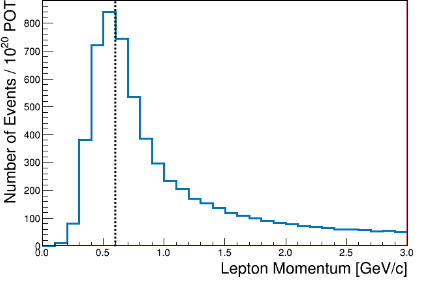
\includegraphics[width=0.48\textwidth]{Chapters/Figures/P0DBANFFParameterization/MomentumKinematicsNumuCC1Track}}\subfloat[Momentum resolution]{\centering{}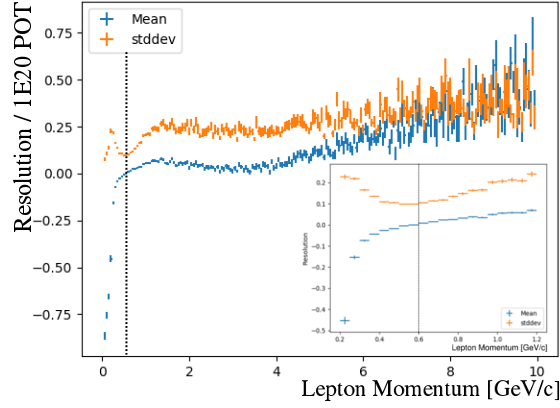
\includegraphics[width=0.45\textwidth]{Chapters/Figures/P0DBANFFParameterization/MomentumKinematicsUncertaintiesNumuCC1Track}}
\par\end{centering}
\caption[Main Track Momentum Resolution for the $\numu$ in FHC Mode CC 1-Track
Sample]{Main track momentum resolution for the $\protect\numu$ in FHC Mode
CC 1-Track sample. Only correctly identified muons are used. The number
of events is scaled to $10^{20}$ POT, which is the approximate scale
for all the samples in this analysis. A dashed line indicates the
maximum of the distribution peak from figure (a). The resolution of
the momentum measurement is shown in figure (b) whose error bars are
estimated using bootstrapping. In the inset is the momentum resolution
zoomed near the momentum distribution maximum.\label{fig:MomentumKinematicsBootstrappingNumuCC1Track}}
\end{figure}

The optimal $\cos\theta$ fit bins were determined in a very similar
manner with the momentum fit bins. While the fit bins and physics
are dictated in $\cos\theta$ space, the detector smearing is a function
$\theta$. In addition, since the angle can be nearly zero for the
most forward-going tracks, the resolution was not used to characterize
the angular uncertainties. Instead, the difference (``residual'')
between the true and reconstructed angle $\theta$ with respect to
(wrt) the ND280 Z-axis was analyzed. The same bootstrapping algorithm
described above was used to determine the mean and stddev of the $\theta$
residuals. The main track angular residuals for the $\numu$ in FHC
Mode CC 1-Track sample are shown in \prettyref{fig:AngularKinematicsBootstrappingNumuCC1Track}
to illustrate the results.

\begin{figure}
\begin{centering}
\subfloat[Angular distribution]{\begin{centering}
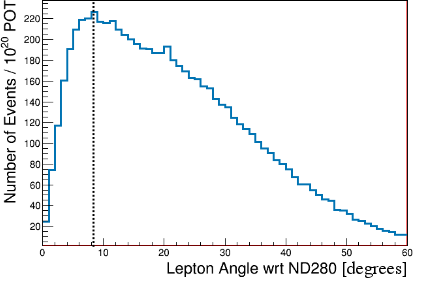
\includegraphics[width=0.475\textwidth]{Chapters/Figures/P0DBANFFParameterization/AngleKinematicsNumuCC1Track}
\par\end{centering}
}\subfloat[Angular residuals]{\begin{centering}
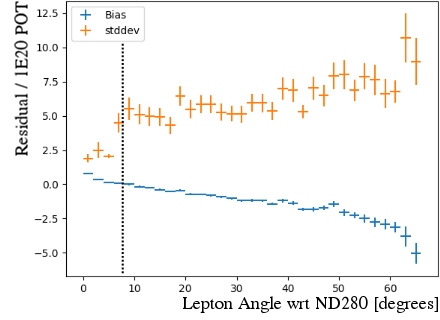
\includegraphics[width=0.45\textwidth]{Chapters/Figures/P0DBANFFParameterization/AngleKinematicsUncertaintiesNumuCC1Track}
\par\end{centering}
}
\par\end{centering}
\caption[Main Track Angular Residuals for the $\numu$ in FHC Mode CC 1-Track
Sample]{Main track angular residuals for the $\protect\numu$ in FHC Mode
CC 1-Track sample. Only correctly identified muons are used. The number
of events is scaled to $10^{20}$ POT, which is the approximate scale
for all the samples in this analysis. A dashed line indicates the
maximum of the distribution peak from figure (a). The residual of
the angular measurement is shown in figure (b) whose error bars are
estimated using bootstrapping. \label{fig:AngularKinematicsBootstrappingNumuCC1Track}}
\end{figure}

This procedure to define fit bin edges emphasizes regions of high
statistics and mitigates regions with low statistics. Since the MC
provides about $10\times$ the data statistics, the statistical uncertainty
for each bin should be negligible in high statistics regions. However,
this does not account for the low statistics regions predicted by
the nominal MC. We tackle this problem and other systematic uncertainties
for the fit bins using bin normalizations as explained in \mbox{Chapter~\ref{chap:BANFF-Likelihood}}. 

\subsection{Fit Bin Edges}

There are a total 988 fit bins with water-in and water-out modes sharing
the same bin edges. The finalized fit bins are tabulated below.
\begin{itemize}
\item The $\numu$ in FHC Mode CC 1-Track water-in and water-out samples:
\begin{itemize}
\item $p$ {[}GeV/c{]}: 0, 0.3, 0.4, 0.5, 0.6, 0.7, 0.8, 1, 1.25, 1.5, 2,
3, 4, 5.5, 30
\item $\cos\theta$ : -1, 0.7, 0.8 , 0.88, 0.94, 0.96, 0.975, 0.99, 1
\end{itemize}
\item The $\numu$ in FHC Mode CC N-Tracks water-in and water-out samples:
\begin{itemize}
\item $p$ {[}GeV/c{]}: 0, 0.4, 0.5, 0.6, 0.7, 0.8, 1, 1.2, 1.5, 1.8, 2.2,
2.7, 3.5, 5, 10, 30
\item $\cos\theta$ : -1, 0.65, 0.77, 0.85, 0.9, 0.94, 0.97, 0.99, 1
\end{itemize}
\item The $\numubar$ in RHC Mode CC 1-Track water-in and water-out samples:
\begin{itemize}
\item $p$ {[}GeV/c{]}: 0, 0.4, 0.5, 0.6, 0.7, 0.8, 1, 1.25, 1.5, 2, 3,
30
\item $\cos\theta$ : -1, 0.82, 0.87, 0.9, 0.93, 0.95, 0.97, 0.99, 1
\end{itemize}
\item The $\numubar$ in RHC Mode CC N-Tracks water-in and water-out samples:
\begin{itemize}
\item $p$ {[}GeV/c{]}: 0, 0.5, 0.9, 1.25, 1.6, 2, 3, 8, 30
\item $\cos\theta$ : -1, 0.8, 0.89, 0.95, 0.97, 0.99, 1
\end{itemize}
\item The $\numu$ in RHC CC 1-Track water-in and water-out samples:
\begin{itemize}
\item $p$ {[}GeV/c{]}: 0, 0.4, 0.6, 0.8, 1.1, 2, 10
\item $\cos\theta$ : -1, 0.78, 0.84, 0.89, 0.92, 0.95, 0.97, 0.98, 0.99,
1
\end{itemize}
\item The $\numu$ in RHC CC N-Tracks water-in and water-out samples:
\begin{itemize}
\item $p$ {[}GeV/c{]}: 0, 0.4, 0.6, 0.8, 1, 1.5, 2, 3, 10
\item $\cos\theta$ : -1, 0.7, 0.8, 0.85, 0.9, 0.94, 0.965, 0.98, 0.99,
1
\end{itemize}
\end{itemize}
%


\section{Systematic Uncertainties and Penalty Terms\label{sec:Systematic-Uncertainties-and}}

This section provides details on the penalty terms, and hence fit
parameters, in the BANFF fit. The cross section and flux penalty terms
in this analysis are identical to the previous near detector constraint
studies\cite{Wret2019,Bienstock2017}. This provides a one-to-one
comparison between the $\pod$-only and FGD-only flux and cross section
predictions. However, due to the different detector technologies between
the $\pod$ and FGD, different bin normalization parameters are necessary.

The fit parameters are described in the following order. The first
set of parameters are the flux terms. This is followed by a description
of the fit bin normalization parameters. The final topic is a description
of the cross section parameters.


\subsection{Flux Model Parameters}

The T2K neutrino flux model is a description of the neutrino beam
energy spectrum for each run period and flavor. This model includes
simulations of the proton beam interactions and subsequent hadron
production at the target. The predicted hadron production rate, including
inside and outside the graphite target, is tuned to the results from
the replica target\footnote{The NA61/SHINE experiment has two graphite targets. A thin 2 cm target
and a thick 90 cm target. The thick target is a replica of the T2K
graphite target.} experiment NA61/SHINE\cite{Abgrall:2016fs} and other hadron production
experiments. The uncertainties in the unoscillated flux tuning are
dominated by hadron production. Smaller effects on the unoscillated
flux uncertainty include the proton beam profile, off-axis angle,
horn current, and horn alignment. Further details about the flux model
and uncertainties can be found in the following reference\cite{Abe:2017vif}.
The flux parameters are especially important since they are used as
inputs to the oscillation analysis. 

The flux penalty term in the BANFF fit is defined as
\begin{equation}
\chi_{\text{Flux}}^{2}=\left(\flux-\flux_{0}\right)^{T}\left(V^{\text{Flux}}\right)^{-1}\left(\flux-\flux_{0}\right),\label{eq:DeltaChi2Flux}
\end{equation}
where $\vec{b}$ is the vector of flux parameter values, $\vec{b}_{0}$
is the vector of the initial parameter values, and $V^{\text{Flux}}$
is the flux covariance matrix. As a remainder, all penalty terms in
this analysis have the form of \eqref{eq:DeltaChi2Flux}. Each flux
parameter is a neutrino energy bin normalization starting at one (1).
Formally, a flux bin is defined as 
\begin{equation}
b_{i}=\frac{N_{\nu_{\alpha},i}^{\prime}}{N_{\nu_{\alpha},i}},\label{eq:fluxtermdef}
\end{equation}
where $N_{\nu_{\alpha},i}$ and $N_{\nu_{\alpha},i}^{\prime}$ are
the predicted and ND constrained $\nu_{\alpha}$ event rates, respectively,
in the $i$th energy bin. In other words, \textit{each flux term is
a ratio of rates}. \textit{Further, all penalty terms and covariance
terms are dimensionless}. A postfit value of 1.1 indicates that all
events in that energy bin have an additional weight of 1.1, signaling
that the postfit prefers to increase that neutrino flux by 10\%. Equivalently,
this means $N_{\nu_{\alpha},i}^{\prime}$ is 10\% greater than $N_{\nu_{\alpha},i}$. 

In the BANFF fit, both ND280 and SK flux parameters are estimated
simultaneously. This is achieved using correlations between ND280
and SK flux parameters in the covariance matrix. The covariance matrix
is provided by the T2K flux group and is shown in \prettyref{fig:BANFF-pre-fit-flux-covariance}.
Also shown in \prettyref{fig:BANFF-pre-fit-flux-covariance} is the
Pearson linear correlation coefficient matrix which is defined as
\begin{equation}
\rho_{i,j}=\frac{V_{i,j}}{\sqrt{V_{i,i}V_{j,j}}},\label{eq:pearson-correlation}
\end{equation}
where $i$ and $j$ are bins in $V$.

\begin{figure}
\centering{}\subfloat[Covariance matrix]{\begin{centering}
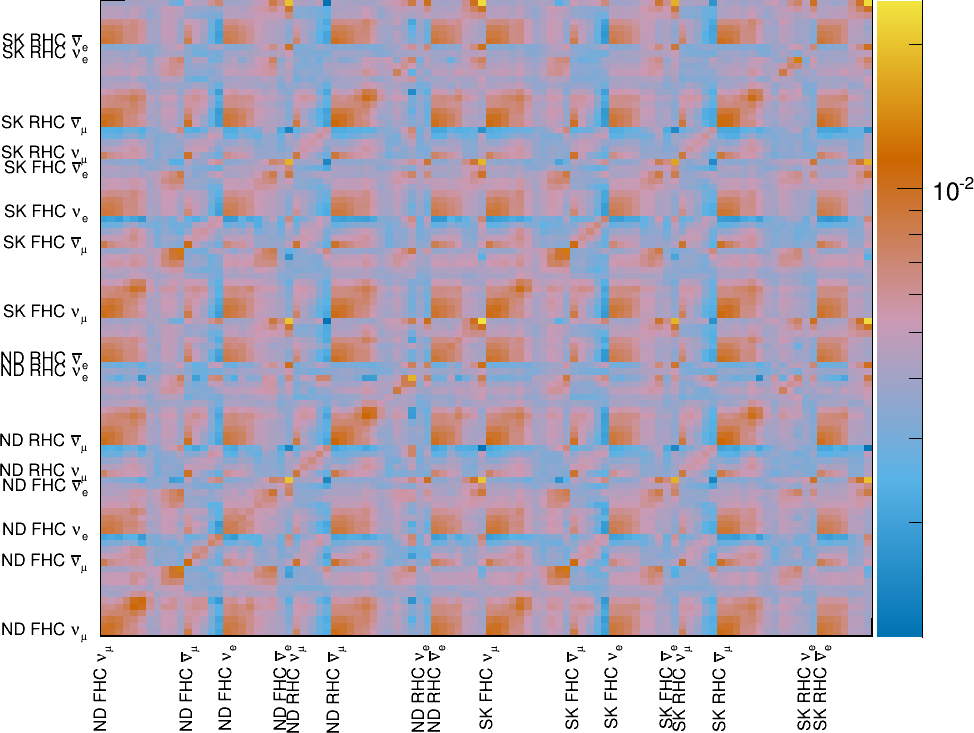
\includegraphics[width=0.45\textwidth]{Chapters/Figures/P0DBANFFParameterization/BANFF_Flux_matrix}
\par\end{centering}
}\subfloat[Correlation matrix]{\begin{centering}
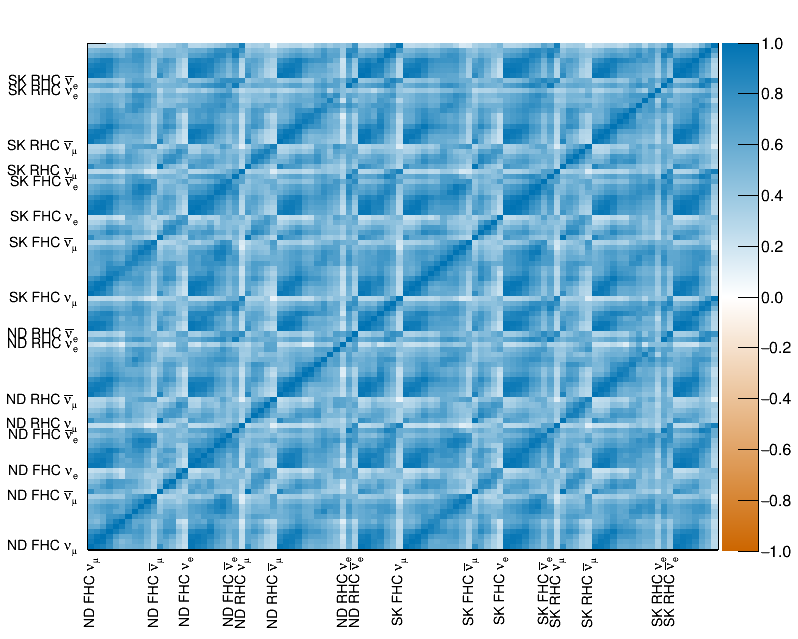
\includegraphics[width=0.45\textwidth]{Chapters/Figures/P0DBANFFParameterization/BANFF_Flux_matrix_corr}
\par\end{centering}
}\caption[The BANFF Prefit Flux Covariance Matrix]{The BANFF prefit flux covariance matrix. Figure (a) is shows the covariance
matrix which is the uncertainty of the normalization for the neutrino
flux at both ND280 and SK. The covariance matrix is divided into submatrices
in groups by detector, beam mode, and neutrino flavor. Figure (b)
is the linear correlation coefficient for each covariance term. \label{fig:BANFF-pre-fit-flux-covariance}}
\end{figure}

\begin{figure}
\begin{centering}
\subfloat[Unoscillated SK FHC flux]{\begin{centering}
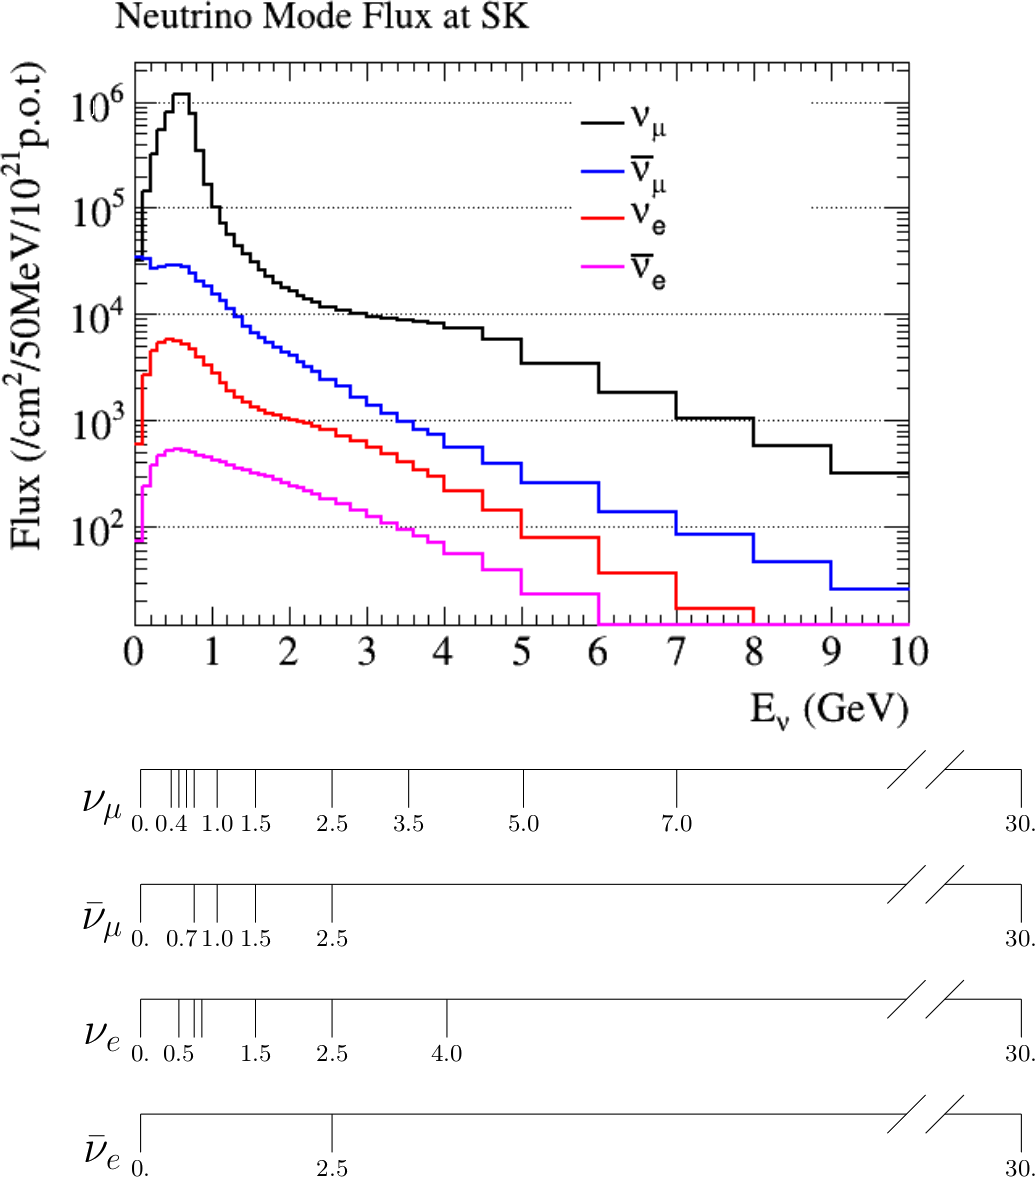
\includegraphics[width=0.45\textwidth]{Chapters/Figures/Systematics/SKFHCFlux}
\par\end{centering}
}\subfloat[Unoscillated SK RHC flux]{\begin{centering}
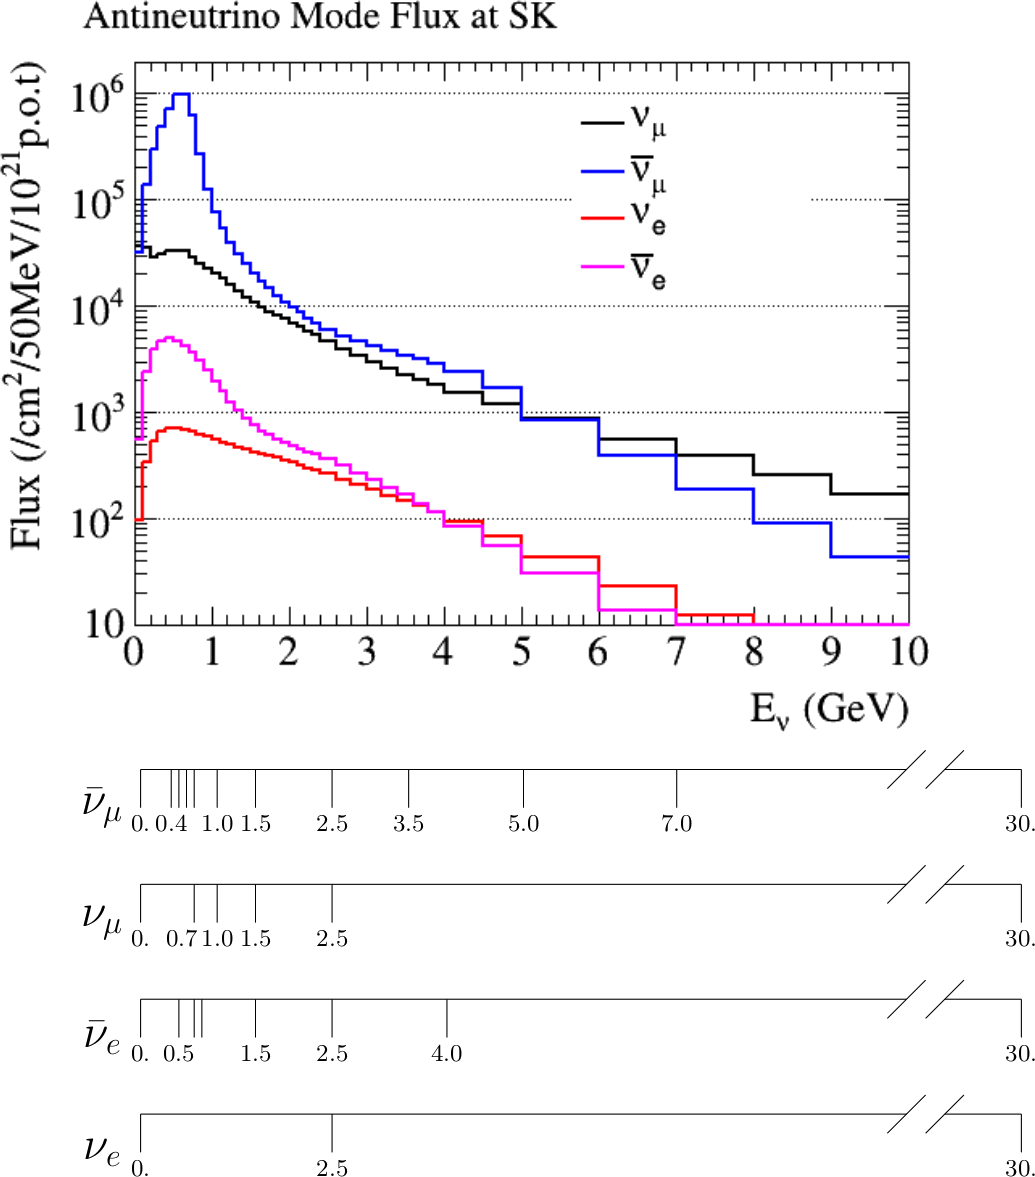
\includegraphics[width=0.45\textwidth]{Chapters/Figures/Systematics/SKRHCFlux}
\par\end{centering}
}
\par\end{centering}
\caption[Neutrino Flux Prediction at SK and Flux Bin Edges]{Neutrino flux prediction at SK and flux bin edges. The flux prediction
for FHC (RHC) mode is shown in figure on the left (right). The flux
normalization parameters have an assigned energy range and are the
same for both the SK and ND280 detectors. The energy binning used
is shown below the plots. \label{fig:UnoscillatedFluxSK}}
\end{figure}

The tabulated flux parameters/bins and uncertainties in this analysis
are given in \prettyref{tab:Fluxbinning}. These are the first set
of parameters in the fit. The flux parameters are differentiated by
neutrino energy, horn current/polarity (FHC mode and RHC mode), neutrino
flavor ($\numu$, $\numubar$, $\nue$, and $\nuebar$), and detector
(ND280 and SK). There are 50 ND280 and 50 SK flux parameters to yield
a total of 100 flux normalizations. In addition, the bin edges are
shared between the ND280 and SK. The SK neutrino flux and the flux
bin edges are shown in \prettyref{fig:UnoscillatedFluxSK}. \newpage{}

\begin{center}
\begin{longtable}[c]{cccc}
\hline
\caption[Flux Binning and Uncertainties]{Flux binning and uncertainties used in the BANFF fit.\label{tab:Fluxbinning}}
\tabularnewline
\textbf{Fit index} & \textbf{Beam mode} & \textbf{Bin edges {[}GeV{]}} & \textbf{Prefit}\tabularnewline
\hline
\endfirsthead
\hline
\tabularnewline
\textbf{Fit index} & \textbf{Beam mode} & \textbf{Bin edges {[}GeV{]}} & \textbf{Prefit}\tabularnewline
\hline
\endhead 
0 & ND280 $\numu$ FHC & 0.0 - 0.4 & 1$\pm$0.100909\tabularnewline
1 &  & 0.4 - 0.5 & 1$\pm$0.099431\tabularnewline
2 &  & 0.5 - 0.6 & 1$\pm$0.092025\tabularnewline
3 &  & 0.6 - 0.7 & 1$\pm$0.085239\tabularnewline
4 &  & 0.7 - 1.0 & 1$\pm$0.105356\tabularnewline
5 &  & 1.0 - 1.5 & 1$\pm$0.104375\tabularnewline
6 &  & 1.5 - 2.5 & 1$\pm$0.073612\tabularnewline
7 &  & 2.5 - 3.5 & 1$\pm$0.068993\tabularnewline
8 &  & 3.5 - 5.0 & 1$\pm$0.082334\tabularnewline
9 &  & 5.0 - 7.0 & 1$\pm$0.097308\tabularnewline
10 &  & 7.0 - 30 & 1$\pm$0.114706\tabularnewline
11 & ND280 $\numubar$ FHC & 0.0 - 0.7 & 1$\pm$0.103804\tabularnewline
12 &  & 0.7 - 1.0 & 1$\pm$0.084158\tabularnewline
13 &  & 1.0 - 1.5 & 1$\pm$0.081349\tabularnewline
14 &  & 1.5 - 2.5 & 1$\pm$0.085208\tabularnewline
15 &  & 2.5 - 30 & 1$\pm$0.087735\tabularnewline
16 & ND280 $\nue$ FHC & 0.0 - 0.5 & 1$\pm$0.091336\tabularnewline
17 &  & 0.5 - 0.7 & 1$\pm$0.089699\tabularnewline
18 &  & 0.7 - 0.8 & 1$\pm$0.084648\tabularnewline
19 &  & 0.8 - 1.5 & 1$\pm$0.079722\tabularnewline
20 &  & 1.5 - 2.5 & 1$\pm$0.079766\tabularnewline
21 &  & 2.5 - 4.0 & 1$\pm$0.081399\tabularnewline
22 &  & 4.0 - 30 & 1$\pm$0.095795\tabularnewline
23 & ND280 $\nuebar$ FHC & 0.0 - 2.5 & 1$\pm$0.072069\tabularnewline
24 &  & 2.5 - 30 & 1$\pm$0.142921\tabularnewline
25 & ND280 $\numu$ RHC & 0.0 - 0.7 & 1$\pm$0.094066\tabularnewline
26 &  & 0.7 - 1.0 & 1$\pm$0.079866\tabularnewline
27 &  & 1.0 - 1.5 & 1$\pm$0.080948\tabularnewline
28 &  & 1.5 - 2.5 & 1$\pm$0.083251\tabularnewline
29 &  & 2.5 - 30 & 1$\pm$0.082653\tabularnewline
30 & ND280 $\numubar$ RHC & 0.0 - 0.4 & 1$\pm$0.107277\tabularnewline
31 &  & 0.4 - 0.5 & 1$\pm$0.098851\tabularnewline
32 &  & 0.5 - 0.6 & 1$\pm$0.089710\tabularnewline
33 &  & 0.6 - 0.7 & 1$\pm$0.084692\tabularnewline
34 &  & 0.7 - 1.0 & 1$\pm$0.106871\tabularnewline
35 &  & 1.0 - 1.5 & 1$\pm$0.098711\tabularnewline
36 &  & 1.5 - 2.5 & 1$\pm$0.073350\tabularnewline
37 &  & 2.5 - 3.5 & 1$\pm$0.070520\tabularnewline
38 &  & 3.5 - 5.0 & 1$\pm$0.092905\tabularnewline
39 &  & 5.0 - 7.0 & 1$\pm$0.089083\tabularnewline
40 &  & 7.0 - 30 & 1$\pm$0.134911\tabularnewline
41 & ND280 $\nue$ RHC & 0.0 - 2.5 & 1$\pm$0.066214\tabularnewline
42 &  & 2.5 - 30 & 1$\pm$0.086977\tabularnewline
43 & ND280 $\nuebar$ RHC & 0.0 - 0.5 & 1$\pm$0.095575\tabularnewline
44 &  & 0.5 - 0.7 & 1$\pm$0.089033\tabularnewline
45 &  & 0.7 - 0.8 & 1$\pm$0.088406\tabularnewline
46 &  & 0.8 - 1.5 & 1$\pm$0.081472\tabularnewline
47 &  & 1.5 - 2.5 & 1$\pm$0.078353\tabularnewline
48 &  & 2.5 - 4.0 & 1$\pm$0.089427\tabularnewline
49 &  & 4.0 - 30 & 1$\pm$0.156972\tabularnewline
50 & SK $\numu$ FHC & 0.0 - 0.4 & 1$\pm$0.102555\tabularnewline
51 &  & 0.4 - 0.5 & 1$\pm$0.101771\tabularnewline
52 &  & 0.5 - 0.6 & 1$\pm$0.092573\tabularnewline
53 &  & 0.6 - 0.7 & 1$\pm$0.084265\tabularnewline
54 &  & 0.7 - 1.0 & 1$\pm$0.102271\tabularnewline
55 &  & 1.0 - 1.5 & 1$\pm$0.084528\tabularnewline
56 &  & 1.5 - 2.5 & 1$\pm$0.066909\tabularnewline
57 &  & 2.5 - 3.5 & 1$\pm$0.072355\tabularnewline
58 &  & 3.5 - 5.0 & 1$\pm$0.085299\tabularnewline
59 &  & 5.0 - 7.0 & 1$\pm$0.096725\tabularnewline
60 &  & 7.0 - 30 & 1$\pm$0.114112\tabularnewline
61 & SK $\numubar$ FHC & 0.0 - 0.7 & 1$\pm$0.103129\tabularnewline
62 &  & 0.7 - 1.0 & 1$\pm$0.078327\tabularnewline
63 &  & 1.0 - 1.5 & 1$\pm$0.082367\tabularnewline
64 &  & 1.5 - 2.5 & 1$\pm$0.082121\tabularnewline
65 &  & 2.5 - 30 & 1$\pm$0.085123\tabularnewline
66 & SK $\nue$ FHC & 0.0 - 0.5 & 1$\pm$0.090918\tabularnewline
67 &  & 0.5 - 0.7 & 1$\pm$0.087065\tabularnewline
68 &  & 0.7 - 0.8 & 1$\pm$0.082527\tabularnewline
69 &  & 0.8 - 1.5 & 1$\pm$0.076514\tabularnewline
70 &  & 1.5 - 2.5 & 1$\pm$0.075773\tabularnewline
71 &  & 2.5 - 4.0 & 1$\pm$0.082078\tabularnewline
72 &  & 4.0 - 30 & 1$\pm$0.092882\tabularnewline
73 & SK $\nuebar$ FHC & 0.0 - 2.5 & 1$\pm$0.071921\tabularnewline
74 &  & 2.5 - 30 & 1$\pm$0.128982\tabularnewline
75 & SK $\numu$ RHC & 0.0 - 0.7 & 1$\pm$0.093954\tabularnewline
76 &  & 0.7 - 1.0 & 1$\pm$0.076369\tabularnewline
77 &  & 1.0 - 1.5 & 1$\pm$0.074900\tabularnewline
78 &  & 1.5 - 2.5 & 1$\pm$0.078108\tabularnewline
79 &  & 2.5 - 30 & 1$\pm$0.077505\tabularnewline
80 & SK $\numubar$ RHC & 0.0 - 0.4 & 1$\pm$0.108593\tabularnewline
81 &  & 0.4 - 0.5 & 1$\pm$0.101912\tabularnewline
82 &  & 0.5 - 0.6 & 1$\pm$0.092787\tabularnewline
83 &  & 0.6 - 0.7 & 1$\pm$0.082669\tabularnewline
84 &  & 0.7 - 1.0 & 1$\pm$0.102090\tabularnewline
85 &  & 1.0 - 1.5 & 1$\pm$0.087732\tabularnewline
86 &  & 1.5 - 2.5 & 1$\pm$0.068117\tabularnewline
87 &  & 2.5 - 3.5 & 1$\pm$0.069902\tabularnewline
88 &  & 3.5 - 5.0 & 1$\pm$0.091711\tabularnewline
89 &  & 5.0 - 7.0 & 1$\pm$0.084736\tabularnewline
90 &  & 7.0 - 30 & 1$\pm$0.115488\tabularnewline
91 & SK $\nue$ RHC & 0.0 - 2.5 & 1$\pm$0.066204\tabularnewline
92 &  & 2.5 - 30 & 1$\pm$0.082645\tabularnewline
93 & SK $\nuebar$ RHC & 0.0 - 0.5 & 1$\pm$0.095453\tabularnewline
94 &  & 0.5 - 0.7 & 1$\pm$0.088889\tabularnewline
95 &  & 0.7 - 0.8 & 1$\pm$0.085644\tabularnewline
96 &  & 0.8 - 1.5 & 1$\pm$0.078536\tabularnewline
97 &  & 1.5 - 2.5 & 1$\pm$0.075246\tabularnewline
98 &  & 2.5 - 4.0 & 1$\pm$0.086384\tabularnewline
99 &  & 4.0 - 30 & 1$\pm$0.152507\tabularnewline
\hline
\end{longtable}
\par\end{center}


\subsection{Detector Inefficiencies And Bins Normalization Parameters}

In the BANFF fit, fit bin normalization parameters are used to penalize
variations in the fit bins. Varying fit bins without constraint is
nonphysical due to known detector inefficiencies and their systematic
uncertainties. This information is incorporated into the penalty term,
$\chi_{\text{Det}}^{2}$. Since improperly modeled inefficiencies
can cause events to migrate from bin-to-bin, numerous fake ``toy
experiments'' are performed to evaluate the systematic uncertainties
in detector inefficiencies. When all toy experiments are analyzed
together, correlated variations among fit bins become apparent. These
correlations provide the constraints on freely changing bin normalizations.
We will see the result of running such toy experiment variations in
the coming pages. Hitherto in this technote, detector inefficiency
uncertainties will be referred to as detector systematics.

All the detector systematics are evaluated either as observable variations
or weights. An observable variation affects the physical observables
of selected events like the calculated energy loss of a track in the
$\pod$. A weight is a multiplicative factor that alters the normalization
of a single event in a bin. There are detector systematics that affect
the $\pod$-only, TPC-only, or both.

This section is organized as follows. The systematics treatment model
for the detector systematics developed to evaluate their effects on
the analysis is described in \mbox{Section~\ref{subsec:Systematic-Treatment-Models}}.
The specific systematic uncertainties relevant to this analysis are
described in \mbox{Section~\ref{subsec:Detector-Systematics}}. The
detector systematics penalty term used in the BANFF fit is described
in \mbox{Section~\ref{subsec:Detector-Systematics-Penalty}}. Finally,
the procedure to determine the initial bin normalization is presented
in \mbox{Section~\ref{subsec:Bin-Normalization-Parameters}}.

\subsubsection{Systematic Treatment Models\label{subsec:Systematic-Treatment-Models}}

The BANFF fit analysis uses toy experiment variations to evaluate
the effect of detector systematics on the analysis samples. Each toy
experiment loops over all the predicted events and varies the known
detector systematic effects. Each systematic effect either varies
the event's efficiency weight or event observables. Both the observable
variation and efficiency-like weight treatments rely on data-driven
studies by comparing data and MC predictions in a control sample\footnote{Each control sample is validated in T2K prior to introduction to the
BANFF analysis.} (CS). By using a large ensemble of toy experiments, the effect of
the detector systematics on the samples is evaluated. 

Efficiency-like corrections alter the number of predicted events in
a fit bin. The model used to evaluate efficiency-like systematics
is given by
\begin{equation}
\epsilon_{\text{Data}}(o)=\left(\frac{\epsilon_{\text{Data}}(o)}{\epsilon_{\text{MC}}(o)}\right)_{\text{CS}}\epsilon_{\text{MC}}(o),\label{eq:effdatafromCS}
\end{equation}
where $\epsilon_{\text{MC}}/\epsilon_{\text{Data}}$ denotes the mean
selection efficiency of the MC/data as a function of some observable
kinematic $o$, and $\left(\ \right)_{\text{CS}}$ refers to the selection
efficiency measured in a CS. We need to update this model to account
for statistical uncertainties in the CS. The updated model, with $o$
dependence assumed, is now 
\begin{equation}
\epsilon_{\text{Data}}^{\prime}=\left(\frac{\epsilon_{\text{Data}}+x_{\text{Data}}\cdot\sigma_{\epsilon_{\text{Data}}}}{\epsilon_{\text{MC}}+x_{\text{MC}}\cdot\sigma_{\epsilon_{\text{MC}}}}\right)_{\text{CS}}\epsilon_{\text{MC}}\label{eq:effdataWithErrfromCS}
\end{equation}
where $\sigma_{\epsilon_{\text{MC}}}/\sigma_{\epsilon_{\text{Data}}}$
is the standard deviation of the efficiency of the MC/Data and $x_{\text{Data}}$
and $x_{\text{MC}}$ are uncorrelated, random normally distributed
numbers from $\mathcal{N}\left(\mu=0,\sigma^{2}=1\right)$. All the
variations are applied to the event, simultaneously affecting all
observables, and the event selection is rerun. A weight is derived
depending if the event is selected, $w_{\text{eff}}$, or not selected,
$w_{\text{ineff}}$. These weights are given below
\begin{equation}
\begin{aligned}w_{\text{eff}} & =\frac{\epsilon_{\text{Data}}^{\prime}}{\epsilon_{\text{MC}}}\\
w_{\text{ineff}} & =\frac{1-\epsilon_{\text{Data}}^{\prime}}{1-\epsilon_{\text{MC}}}.
\end{aligned}
\label{eq:weighteff}
\end{equation}

Observable variation systematics are evaluated as shifts to physically
measured quantities like particle track momentum and track length.
The systematic can be evaluated in two different ways:
\begin{enumerate}
\item If the reconstructed observable, $o_{\text{reco}}$, has a known true
value, $o_{\text{true}}$, then the difference between those two is
used as scaling. The varied observable is given by
\begin{equation}
o^{\prime}=o_{\text{true}}+\left(o_{\text{reco}}-o_{\text{true}}\right)\left(s+x\sigma_{s}\right),\label{eq:recotrueobsvar}
\end{equation}
where $s$ is the mean scaling parameter used to match the true value,
$\sigma_{s}$ is the uncertainty on $s$, and $x$ is a random number
from $\mathcal{N}\left(\mu=0,\sigma^{2}=1\right)$. The mean scaling
parameter and its uncertainty are determined from the standard deviations
observed in the data and MC by
\begin{equation}
s=\frac{\delta^{\text{data}}}{\delta^{\text{MC}}}\quad\sigma_{s}=s\left|\frac{\sigma_{\delta^{\text{data}}}}{\delta^{\text{data}}}-\frac{\sigma_{\delta^{\text{MC}}}}{\delta^{\text{MC}}}\right|.\label{eq:scalingdefrecotrueobsvar}
\end{equation}
\item If the MC reconstructed observable is corrected to match the mean
from some CS reconstructed observable. The varied observable in this
case is given by
\begin{equation}
o^{\prime}=o_{\text{Nom}}+\Delta o+x\sigma_{\Delta o},\label{eq:obsvariation}
\end{equation}
where $o^{\prime}$ is the varied observable value, $o_{\text{Nom}}$
is the nominal MC value, $\Delta o$ is the average correction to
the observable, $\sigma_{\Delta o}$ is the uncertainty on the correction,
and $x$ is a random, normal number from $\mathcal{N}\left(\mu=0,\sigma^{2}=1\right)$.
\end{enumerate}
Additional uncertainties from the magnetic field are also special
cases of the 2nd observable variation method specifically for the
TPC momentum\cite{Wret2019}. They are:
\begin{itemize}
\item The TPC laser calibration corrections are applied after the magnetic
field (B-field) mapping corrections. The B-field corrections are applied
at event reconstruction while the calibration corrections are treated
as a systematic uncertainty. The varied momentum is given by
\begin{equation}
p^{\prime}=p_{\text{Nom}}+x\left(p_{\text{Map}}-p_{\text{Nom}}\right),\label{eq:obsvariationtpclaser}
\end{equation}
where $p_{\text{Nom}}$ is the nominal MC prediction using the B-field
corrections and $p_{\text{Map}}$ is the updated momentum using the
additional laser calibration mapping.
\item The momentum depends on some scale parameter $s$. The varied momentum
due to the scale uncertainty is given by
\begin{equation}
p^{\prime}=p_{\text{Nom}}\left(1+x\sigma_{s}\right),\label{eq:obsvariationtpcmomentumscale}
\end{equation}
where $\sigma_{s}$ is the uncertainty on the scale. In this parameterization,
$s$ is the scale of the ND280 solenoid current.
\end{itemize}
After all observables are varied and applied to the event, the event
selection cuts are applied again. By doing so after all variations
are applied, the full impact of the systematic on the sample and analysis
bins can be evaluated.

\subsubsection{Detector Systematics\label{subsec:Detector-Systematics}}

Since this analysis uses the $\pod$ and TPC detectors, systematics
that affect both must be included in the toy experiments. The complete
set of detector systematics and their treatment in the analysis are
listed in \prettyref{tab:List-of-detector}. The TPC-only systematics
that have been used in previous BANFF fit analysis are included in
this analysis. Details on the TPC-only systematics are discussed in
the following references\cite{Abe:2017vif,Wret2019}. There are four
$\pod$-only detector systematics that are considered for this BANFF
fit analysis:
\begin{itemize}
\item The $\pod$ detector energy loss scale,
\item The $\pod$ detector energy loss resolution,
\item The $\pod$-TPC inter-detector matching efficiency, and
\item The $\pod$ detector fiducial mass.
\end{itemize}
\begin{table}
\caption[List of Detector Systematics in the Analysis]{List of detector systematics in the analysis. The TPC-only systematics
are discussed in the following reference\cite{Abe:2017vif}. The $\pod$
mass and track matching systematics were not available in the BANFF
framework and treated as uncorrelated additions to the covariance
matrix. \label{tab:List-of-detector}}

\centering{}%
\begin{tabular}{lcl}
\toprule 
Systematic effect & Affected detectors & Treatment\tabularnewline
\midrule
\midrule 
$\pod$ energy loss scale & $\pod$ & observable variation\tabularnewline
$\pod$ energy loss resolution & $\pod$ & observable variation\tabularnewline
$\pod$ mass & $\pod$ & (see text)\tabularnewline
$\pod$-TPC matching eff. & $\pod$, TPC & (see text)\tabularnewline
Pion secondary interactions & $\pod$, TPC & efficiency\tabularnewline
Proton secondary interactions & $\pod$, TPC & efficiency\tabularnewline
Magnetic field distortion & TPC & observable variation\tabularnewline
TPC charge misassignment & TPC & efficiency\tabularnewline
TPC cluster efficiency & TPC & efficiency\tabularnewline
TPC momentum resolution & TPC & observable variation\tabularnewline
TPC momentum scale & TPC & observable variation\tabularnewline
TPC particle identification & TPC & observable variation\tabularnewline
TPC track quality efficiency & TPC & efficiency\tabularnewline
TPC tracking efficiency & TPC & efficiency\tabularnewline
\bottomrule
\end{tabular}
\end{table}

The $\pod$ energy loss scale and resolution affect the measured momentum
in the $\pod$ and are very significant sources of uncertainty. In
the $\numu$ CC-$0\pi$ cross section analysis\cite{PhysRevD.97.012001},
the same selection as the $\numu$ in FHC Mode CC 1-Track selection,
the scale and resolution contributed 1.3\% and 6.7\%, respectively,
to the cross section uncertainty. Those large uncertainties can be
attributed to the design of the $\pod$. It is optimized for $\pi^{0}$
detection as opposed to a dedicated tracking detector like the FGD.
Slight variations in the track reconstruction can significantly alter
the energy loss as measured in \eqref{eq:momentumP0DFull}.

The remaining systematics, the $\pod$ mass and the $\pod$-TPC matching
efficiency, were not available to analyze in toy experiments variations.
They were not implemented in the BANFF framework and unavailable to
implement due to time constraints on this author. Instead, they were
treated as additional uncorrelated systematics on each bin normalization
uncertainty with the normalization value remaining fixed. 

The $\pod$ mass uncertainty is a normalization systematic which affects
the event rate. This is a challenging systematic for analyses of recent
T2K data due to increasingly faulty sensors to measure the water content.
The procedure to fill the water bags required filling them in unison
to prevent uneven bulging. However, faulty sensors would provide poor
quality data, hence bags were under and overfilled. This effect alters
the expected event rate as a function of position.

Another problem with the mass uncertainty is due to structure deformations
in the $\pod$. To understand how the $\pod$ has deformed, it is
important to understand how the $\pod$ is mounted in the ND280 detector.
Each corner of the $\pod$ is mounted to the ND280 basket leaving
the those corners spatially fixed. When the water bags are filled,
the WT volume expands or ``bulges'' from the middle. The upstream
end of the $\pod$, the Upstream ECal, resists deformations since
it is physically against the ND280 support structure and magnet yoke.
The downstream end of the $\pod$, or the Central ECal (CECal), is
free to deform, however, since there is a few centimeters air gap
between it and the TPC. The CECal, which has a design thickness of
304 mm\cite{Assylbekov:2011sh}, was observed to bulge about 7-8 mm
from its center due to WT bulging as well\cite{Toki2016}. 

This left more water volume, and importantly more mass, in the most
downstream water bags compared to the upstream bags. This additional
mass or bulging effect is evident in the vertex distribution as a
function of the Z-position as shown in \prettyref{fig:P0DBulging}.

\begin{figure}
\begin{centering}
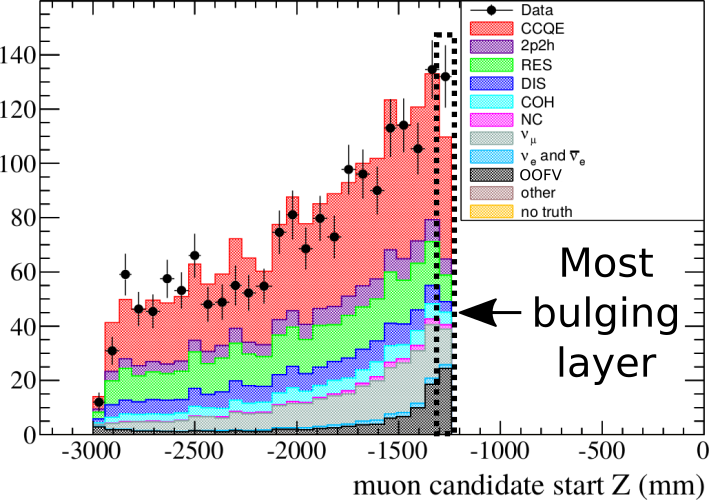
\includegraphics[width=0.45\textwidth]{Chapters/Figures/Systematics/EvidenceOfP0DBulging}
\par\end{centering}
\caption[Vertex Distribution Showing Evidence of \podtitle{} Bulging]{Vertex distribution showing evidence of bulging. In the $\protect\numubar$/$\protect\numu$
cross section ratio analysis, a significant excess of events in the
most downstream layer of the $\pod$ (black, dashed line box) was
observed. Initially thought to be OOFV events, the analyzers removed
the most downstream and upstream layers in their analysis. This distribution
was produced using the run 5, RHC period using selection precuts 1
through 4 and a having a positive track in the TPC. Each event is
categorized by true interaction mode according to NEUT. This figure
was altered for clarity from the following reference \cite{Campbell2017}.\label{fig:P0DBulging}}
\end{figure}

Prior $\pod$ analyses have estimated the mass uncertainty using similar
toy experiment techniques, but did not integrate them into the BANFF
framework. In particular in the $\numu$ in CC-$0\pi$ analysis\cite{PhysRevD.97.012001},
the $\pod$ mass had an 1.5\% systematic effect on the cross section.
Since the $\pod$ mass uncertainty estimate was determined using the
same toy experiment variation method, a conservative estimate of 2\%
on the mass uncertainty is included in this analysis.

The $\pod$ and TPC ($\pod$-TPC) inter-detector track matching efficiency
is estimated to have a small systematic effect on the analysis. It
was analyzed to have over a 99.8\% data and MC efficiency in the single
track $\numu$ CC-$0\pi$ analysis and thus was neglected. However,
since this analysis includes $>1$ track samples, the matching efficiency
for non-single track samples is unknown. The best constraint on multiple
track inter-detector matching is from the private T2K technical note
on the single bin $\numubar/\numu$ cross section analysis \cite{Campbell2017}.
The analysis estimated the uncertainty at less than 0.14\%, albeit
using the ``pre-Global'' technique mentioned in Chapter \ref{chap:P0DSelections}.
Because their track matching algorithm is different than Global's
algorithm, the uncertainty is not guaranteed to remain constant across
the fit bins. A conservative estimate of 1\% for the $\pod$-TPC matching
efficiency was chosen in order to account for the inherent uncertainty
in this systematic.

Now that we know the systematics that affect the analysis, we can
now begin to understand how the detector systematic penalty term $\chi_{\text{Det}}^{2}$
is modeled in the BANFF fit.

\subsubsection{Toy Experiments and the Detector Systematics Penalty\label{subsec:Detector-Systematics-Penalty}}

The bin normalization penalty parameters are restrictions on freely
varying fit bins. To determine the correlations between bins, a large
ensemble of toy experiments is generated. As described in \mbox{Section~\ref{subsec:Systematic-Treatment-Models}},
each toy experiment varies event observables, the momentum and angle
of the main track, and number of events in a fit bin. The bin normalization
parameter for the $i$th bin, or $d_{i}$, is defined as
\begin{equation}
d_{i}=\frac{\left\langle N_{i}\right\rangle _{\text{toys}}}{N_{i}},\label{eq:obsnormdef}
\end{equation}
where $N_{i}$ predicted number of events in fit bin $i$ and $\left\langle N_{i}\right\rangle _{\text{toys}}$
is the average number of events in fit bin $i$ evaluated over all
toy experiments (toys). The predicted event rate for bin $i$ is given
by
\begin{equation}
N_{i}=\sum_{k}^{N_{\text{MC}}}\delta_{i,k}^{\text{bin}}w_{k},\label{eq:bin-nominal}
\end{equation}
where $N_{\text{MC}}$ being the number of unweighted MC events, $\delta_{i,k}^{\text{bin}}$
determines if the $k$th event goes into analysis bin $i$ as a function
of $\left(p,\cos\theta\right)$, and $w_{k}$ is the product of all
of the weights applied to the $k$th event. The weights used in \eqref{eq:bin-nominal}
are 
\begin{equation}
w_{k}=w_{k}^{\text{POT}}\times w_{k}^{\text{Flux}}\times w_{k}^{\text{xsec}}\times w_{k}^{\text{Det}},\label{eq:EventWeights}
\end{equation}
(see \eqref{eq:n-predicted-BANFF} for all possible weights). The
number of events in fit bin $i$, averaged over all toy experiments
(toys), is given by 
\begin{equation}
\begin{aligned}\left\langle N_{i}\right\rangle _{\text{toys}} & =\frac{1}{N_{\text{toys}}}\sum_{t=1}^{N_{\text{toys}}}\left(N_{i}\right)_{t}\\
 & =\frac{1}{N_{\text{toys}}}\sum_{t=1}^{N_{\text{toys}}}\left(\sum_{k}^{N_{\text{MC}}}\left[\delta_{i,k}^{\text{bin}}w_{k}\right]\right)_{t},
\end{aligned}
\label{eq:NAvgToys}
\end{equation}
where now each MC event has a toy variation out of $N_{\text{toys}}$
total toys. We average the results of the toys to smooth out variations
among all toy experiments. In this analysis, and in previous BANFF
analyses as well, $N_{\text{toys}}=2000$ toys were generated as to
have a small sample size uncertainty.

As stated before, all the penalty parameters are dimensionless and
the detector systematics covariance matrix must be constructed carefully.
The bin-to-bin event rate covariance, $V_{i,j}^{\text{Cov}}$, between
bins $i$ and $j$ is
\begin{equation}
\begin{aligned}V_{i,j}^{\text{Cov}} & =\frac{1}{N_{\text{toys}}}\sum_{t=1}^{N_{\text{toys}}}\left(\left(N_{i}\right)_{t}-\left\langle N_{i}\right\rangle _{\text{toys}}\right)\left(\left(N_{j}\right)_{t}-\left\langle N_{j}\right\rangle _{\text{toys}}\right),\end{aligned}
\label{eq:detector-cov-terms}
\end{equation}
where $\left(N_{i}\right)_{t}$ is defined in \eqref{eq:NAvgToys}.
We also need to account for statistical uncertainties in the fit bins,
and so let us define $V_{i,j}^{\text{Stat}}$ as
\begin{equation}
V_{i,j}^{\text{Stat}}=\text{\ensuremath{\delta_{i,j}}}\sum_{k}^{N^{\text{MC}}}\delta_{i,k}^{\text{bin}}w_{k}^{2},\label{eq:detector-stat-terms}
\end{equation}
where $\delta_{i,j}$ is the Kronecker delta function. In order to
incorporate $V_{i,j}^{\text{Cov}}$ and $V_{i,j}^{\text{Stat}}$ uncertainties,
the total detector covariance matrix, $V_{i,j}^{\text{Det}}$, in
the BANFF fit is defined as 
\begin{equation}
V_{i,j}^{\text{Det}}=\frac{V_{i,j}^{\text{Cov}}+V_{i,j}^{\text{Stat}}}{N_{i}N_{j}},\label{eq:totaldetectorcovariance}
\end{equation}
which is indeed dimensionless as required by \eqref{eq:obsnormdef}
since we divided out the predicted event rate in bins $i$ and $j$.

As stated before, the $\pod$ mass and track matching efficiency systematics
are treated as uncorrelated systematics. In order to propagate their
systematic uncertainties into the analysis, the detector covariance
matrix given in \eqref{eq:totaldetectorcovariance} needs to be updated.
The updated covariance matrix is given by 
\begin{equation}
V_{i,j}^{\text{Det}}\leftarrow\left(\widetilde{V}_{i,j}^{\text{Det}}+\widetilde{\sigma}_{\text{Mass}}^{2}+\widetilde{\sigma}_{\text{Match}}^{2}\right)d_{i}d_{j},\label{eq:covarupdatefrac}
\end{equation}
where $\widetilde{V}_{i,j}^{\text{Det}}$ is the fractional covariance
\begin{equation}
\widetilde{V}_{i,j}^{\text{Det}}=\frac{V_{i,j}^{\text{Det}}}{d_{i}d_{j}},\label{eq:fractionalcovariance}
\end{equation}
$d_{i}$/$d_{j}$ are the bin normalization parameters, and $\widetilde{\sigma}_{\text{Mass}}^{2}=2\%$
and $\widetilde{\sigma}_{\text{Match}}^{2}=1\%$ are the $\pod$ mass
and $\pod$-TPC matching efficiency systematic uncertainties, respectively,
estimated in \mbox{Section~\ref{subsec:Detector-Systematics}}. Together,
the two additional sources of uncertainty increase each term in the
covariance matrix by $0.0005d_{i}d_{j}$. Specifically, the uncertainty
in all the bin normalization parameters (square-root of the diagonal
terms in the covariance matrix) increases by about $2.23\%$. The
updated detector covariance matrix now accounts for the $\pod$ mass
and TPC matching inefficiency systematics.

The penalty term, $\chi_{\text{Det}}^{2}$, in the fit is given by
\begin{equation}
\chi_{\text{Det}}^{2}=\left(\systematics-\vec{d_{0}}\right)^{T}\left(V^{\text{Det}}\right)^{-1}\left(\systematics-\vec{d_{0}}\right)^{T},\label{eq:DetPenalty}
\end{equation}
where $\vec{d_{0}}$ is the initial values of the parameters, and
$V^{\text{Det}}$ is given by \eqref{eq:covarupdatefrac}.

\subsubsection{Bin Normalization Parameters\label{subsec:Bin-Normalization-Parameters}}

While there could be one observable normalization for each analysis
bin, a single normalization can be assigned to multiple analysis bins.
The purpose is to reduce the number of fit parameters since the time
to fit increases non-linearly with the number of fit parameters and
events. Previously, the observable normalization edges were determined
by combining fit bins with ``similar'' covariance. This method proved
problematic since the fit bins with relatively higher statistics were
shared with the same observable normalization parameter. This left
the remaining low statistics regions of $(p,\cos\theta)$ phase space
more susceptible to systematic variations in the toy experiments.

A new procedure was developed to improve the shortcomings of old procedure
which required careful consideration of the statistical uncertainties
and variations between observable normalization prefit values. This
procedure can be imagined as reducing the number of contours in a
topographic map while considering external constraints from other
sensing data. The first step in the procedure is to initialize all
of the observable normalization bin edges to be the same as the fit
bin edges. All steps after this are performed iteratively.

Starting with observable normalization bin with the highest statistics,
a decision is made to merge it with all immediate adjacent bins. If
the individual fractional errors differ significantly before the merge,
do not merge them. In this analysis, a factor of 10 in fractional
uncertainty was determined to sufficiently describe bin similarity
by using values larger and smaller than 10 and observing no significant
differences in the end result. Additionally if the two unmerged bin
normalizations differ by more than 10\%, perform the bin merging.
This step serves to smooth out the observable normalization prefit
space. The procedure is also written in pseudocode in Algorithm \prettyref{alg:binedges}.

\begin{algorithm}
\SetKwData{MaxNorm}{max\_norm}
\SetKwData{MinNorm}{min\_norm}
\SetKwData{D}{d}
\SetKwData{F}{f}
\SetKwData{Redo}{redo}
\SetKwData{False}{\textbf{False}}
\SetKwData{True}{\textbf{True}}
\SetKwData{Dprime}{$\text{d}^\prime$}
\Repeat{\Redo is \False}
{
\Redo $\leftarrow$ \False\;
\For(//sorted from min to max $\delta\%$){each normalization bin \D}
{
  \For{each neighboring analysis bin \F}
  {
    \Dprime $\leftarrow$ normalization bin assigned to \F\;
    \If{\Dprime is same as \D}
    {
      Continue to next analysis bin\;
    }
    \If{$\delta\%(\D) \geq 10 \times \delta\%(\Dprime)$}
    {
      \D is assigned as normalization bin for \F\;
      \Redo $\leftarrow$ \True\;
      Continue to next analysis bin\;
    }
    \MaxNorm  $\leftarrow$ max(norm(\D), norm(\Dprime))\;
    \MinNorm $\leftarrow$ min(norm(\D), norm(\Dprime))\;
    \If{\MaxNorm $\geq 1.1 \times$ \MinNorm}
    {
      \D is assigned as normalization bin for \F\;
      \Redo $\leftarrow$ \True\;
    }
  }
}
Recalculate bin normalizations\;
}

\caption[Algorithm to Merge Normalization Bins]{Algorithm to merge normalization bins. The ``$\delta\%$'' operator
returns the fractional statistical uncertainty for the bin. Since
multiple fit bins can be assigned to a single normalization bin, the
statistics of all fits bins are included. The ``norm'' operator
returns the normalization value for a normalization bin determined
by \eqref{eq:bin-nominal}. Finally, the min/max functions return
the minimum/maximum element in a tuple, respectively. \label{alg:binedges}}
\end{algorithm}

The results of the procedure are shown visually in \prettyref{fig:Bin-normalization-edgesNumuFHC},
\prettyref{fig:Bin-normalization-edgesNumubarRHC}, and \prettyref{fig:Bin-normalization-edgesNuMuRHC}.
While the problem of the highest statistics bins being assigned to
a single observable normalization parameter is still present, fluctuations
between adjacent observable normalization parameters is iteratively
minimized. 

A considerable drawback to using toy experiments to estimate the bin
normalization values and covariance matrix is that not all detector
systematics affect the fit observables $(p,\cos\theta)$ in the same
way. There are non-symmetric systematics and they are especially non-Gaussian
in their effects. Therefore, the covariance matrix from \eqref{eq:totaldetectorcovariance}
is not an exact representation of the detector systematics. To demonstrate
this, results of varied number of events are shown in \prettyref{fig:Representative-event-variations}.
However, the bin normalization standard deviations are very wide and
able to effectively cover the range of possible bin normalizations,
which minimizes the non-Gaussian effects of the systematic. All the
varied toy experiment results are provided in Appendix \prettyref{app:NSigmaVariations}.

\begin{figure}
\subfloat[The $\protect\numu$ in FHC Mode CC 1-Track sample]{\begin{centering}
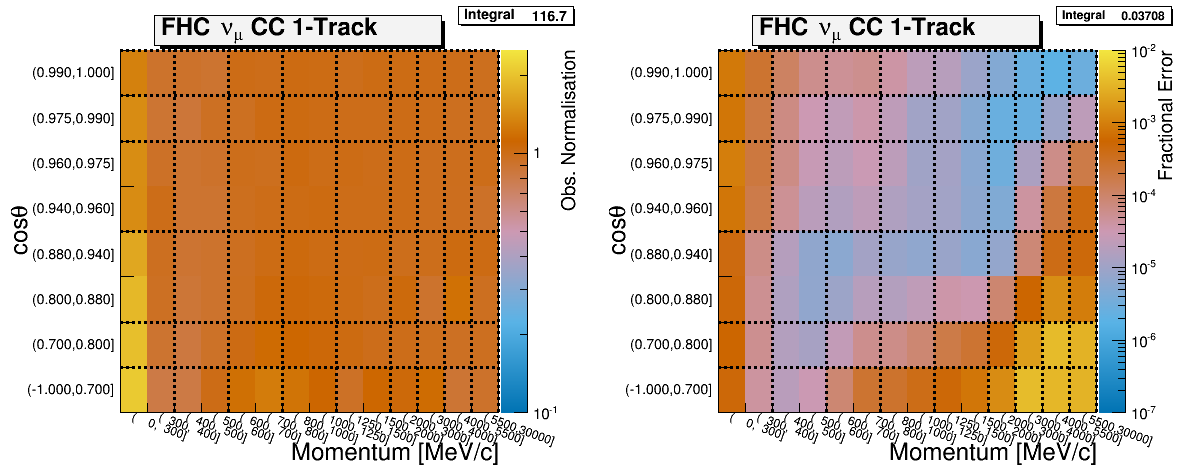
\includegraphics[width=0.95\textwidth]{Chapters/Figures/P0DBANFFParameterization/obsnorm/air/P0DFHCNumuCC1Tr}
\par\end{centering}
}

\subfloat[The $\protect\numu$ in FHC Mode CC N-Tracks sample]{\begin{centering}
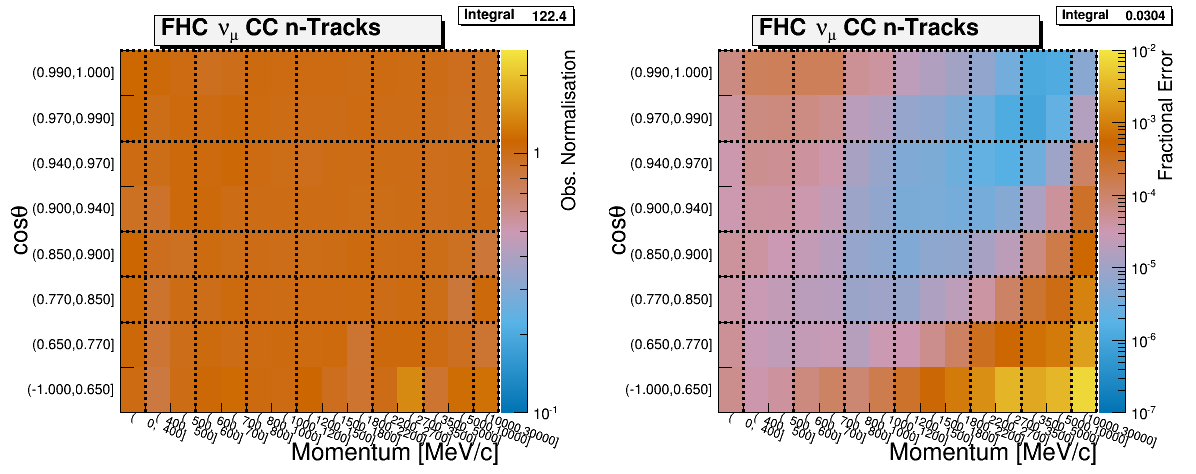
\includegraphics[width=0.95\textwidth]{Chapters/Figures/P0DBANFFParameterization/obsnorm/air/P0DFHCNumuCCnTr}
\par\end{centering}
}

\caption[Bin Normalizations Edges for the $\numu$ in FHC Mode Samples]{Bin normalization edges for the $\protect\numu$ in FHC Mode samples.
The left and right plots show the bin normalization and the bin statistical
fractional error, respectively, if each fit bin had a single bin normalization.
The dashed lines indicate the edges of the bin normalization parameters
finalized for this analysis. Water-in and water-out modes are qualitatively
the same. \label{fig:Bin-normalization-edgesNumuFHC}}
\end{figure}

\begin{figure}
\subfloat[The $\protect\numubar$ in RHC Mode CC 1-Track sample]{\begin{centering}
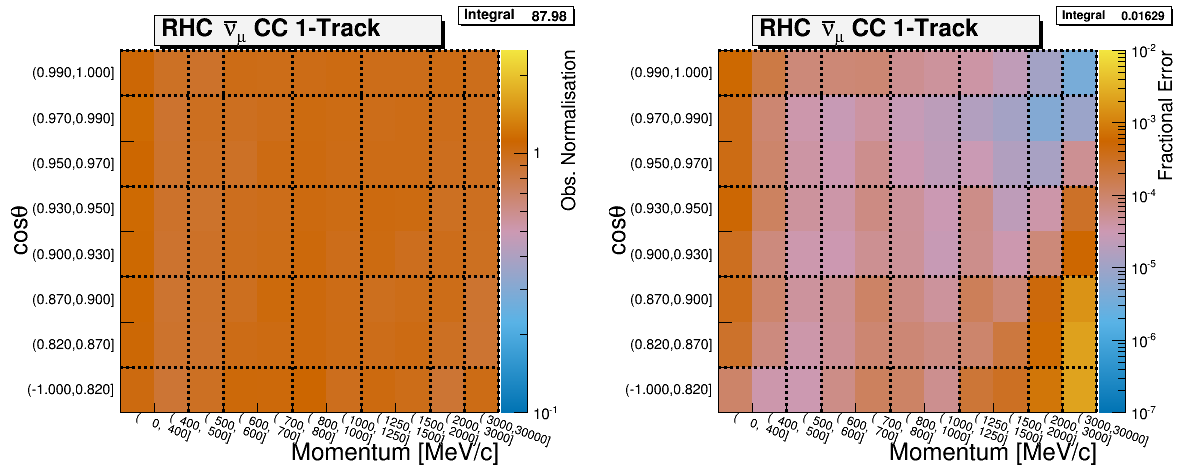
\includegraphics[width=0.95\textwidth]{Chapters/Figures/P0DBANFFParameterization/obsnorm/air/P0DRHCANumuCC1Tr}
\par\end{centering}
}

\subfloat[The $\protect\numubar$ in RHC Mode CC N-Tracks sample]{\begin{centering}
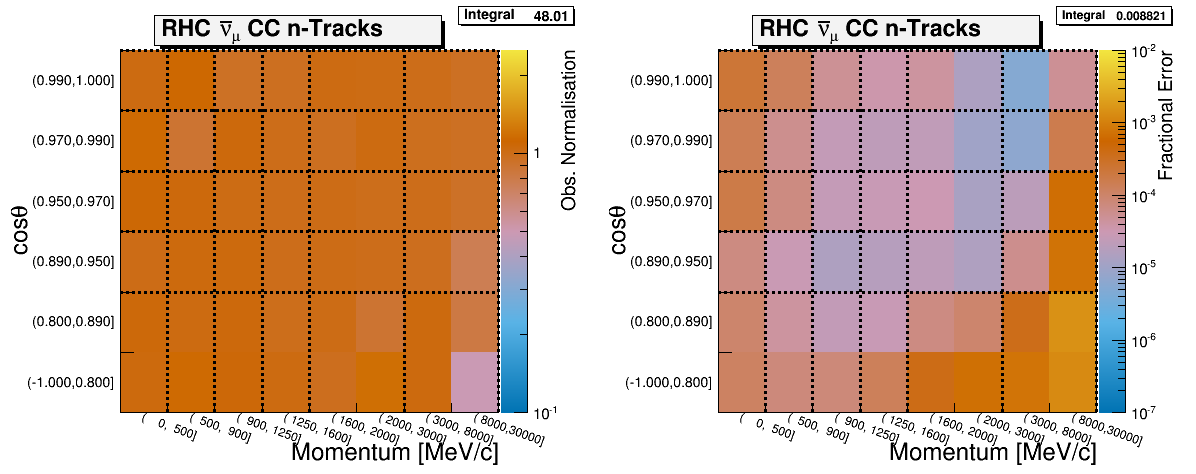
\includegraphics[width=0.95\textwidth]{Chapters/Figures/P0DBANFFParameterization/obsnorm/air/P0DRHCANumuCCnTr}
\par\end{centering}
}

\caption[Bin Normalization Edges for the $\numubar$ in RHC Mode Samples]{Bin normalization edges for the $\protect\numubar$ in RHC Mode samples.
The left and right plots show the bin normalization and the bin statistical
fractional error, respectively, if each fit bin had a single bin normalization.
The dashed lines indicate the edges of the bin normalization parameters
finalized for this analysis. Water-in and water-out modes are qualitatively
the same. \label{fig:Bin-normalization-edgesNumubarRHC}}
\end{figure}

\begin{figure}
\subfloat[The $\protect\numu$ in RHC CC 1-Track sample]{\begin{centering}
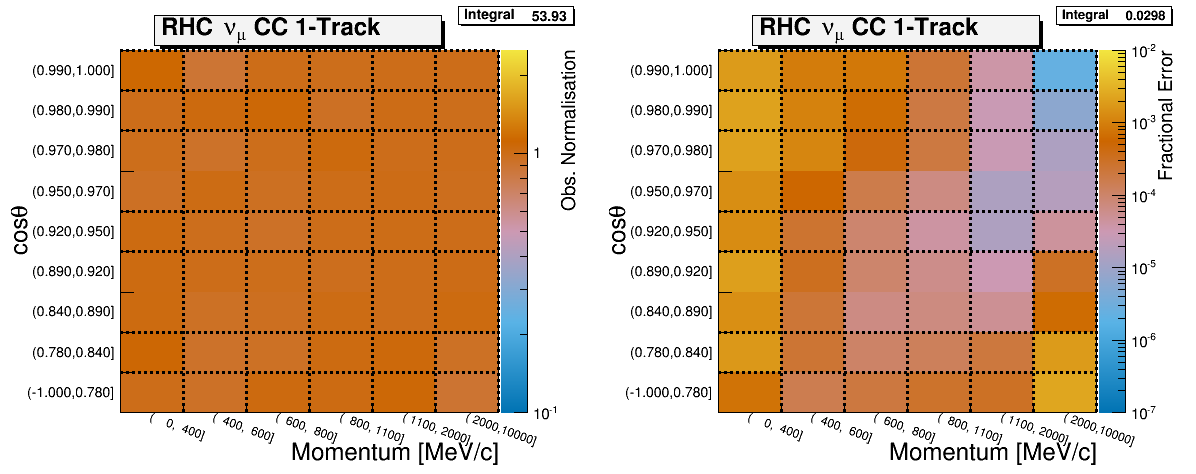
\includegraphics[width=0.95\textwidth]{Chapters/Figures/P0DBANFFParameterization/obsnorm/air/P0DRHCNumuCC1Tr}
\par\end{centering}
}

\subfloat[The $\protect\numu$ in RHC CC N-Tracks sample]{\begin{centering}
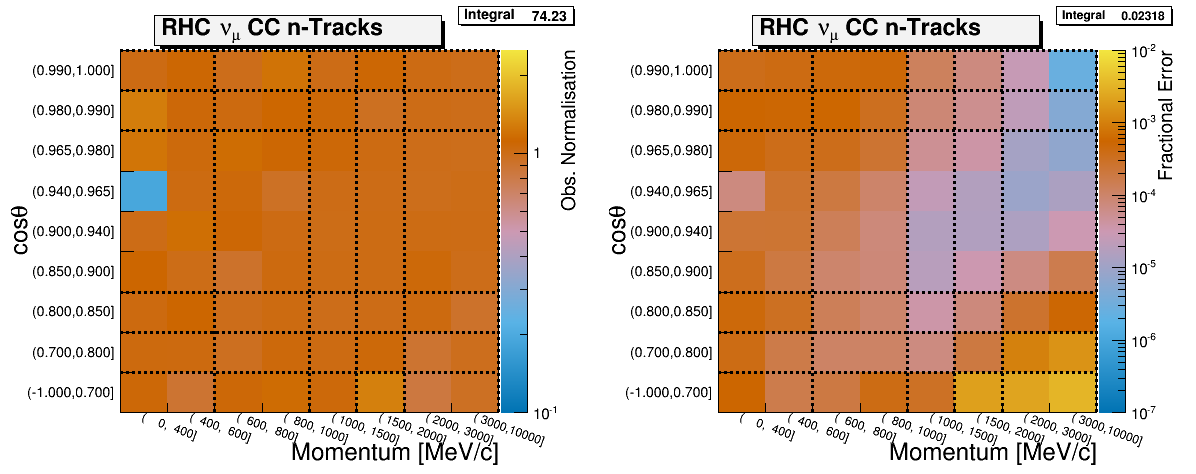
\includegraphics[width=0.95\textwidth]{Chapters/Figures/P0DBANFFParameterization/obsnorm/air/P0DRHCNumuCCnTr}
\par\end{centering}
}

\caption[Bin Normalizations for the $\numu$ Background in RHC Mode Samples]{Bin normalization edges for the $\protect\numu$ Background in RHC
Mode samples. The left and right plots show the bin normalization
and the bin statistical fractional error, respectively, if each fit
bin had a single bin normalization. The dashed lines indicate the
edges of the bin normalization parameters finalized for this analysis.
Water-in and water-out modes are qualitatively the same.\label{fig:Bin-normalization-edgesNuMuRHC}}
\end{figure}

\begin{figure}
\begin{centering}
\subfloat[$\protect\numu$ in FHC CC 1-Track]{\begin{centering}
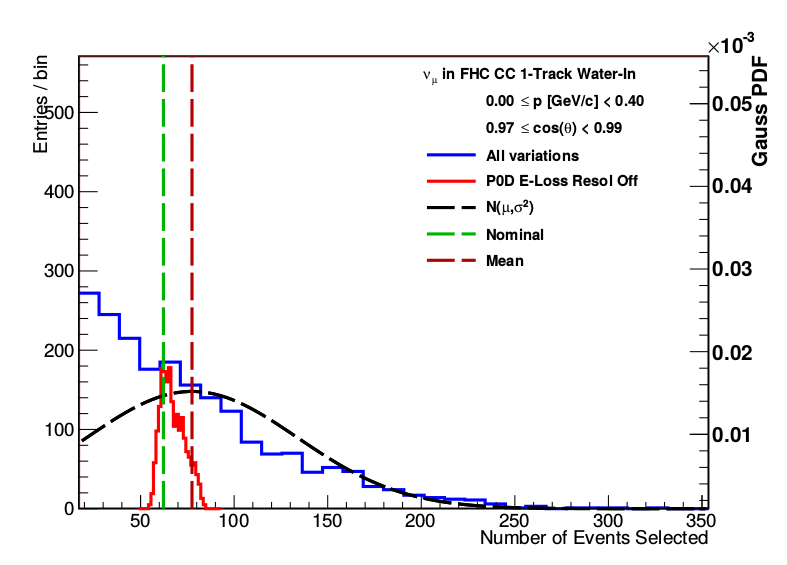
\includegraphics[width=0.445\textwidth]{Chapters/Figures/P0DBANFFParameterization/P0DObsnormSpreadNumuCC1Trk}
\par\end{centering}
}\subfloat[$\protect\numu$ in FHC CC N-Tracks]{\begin{centering}
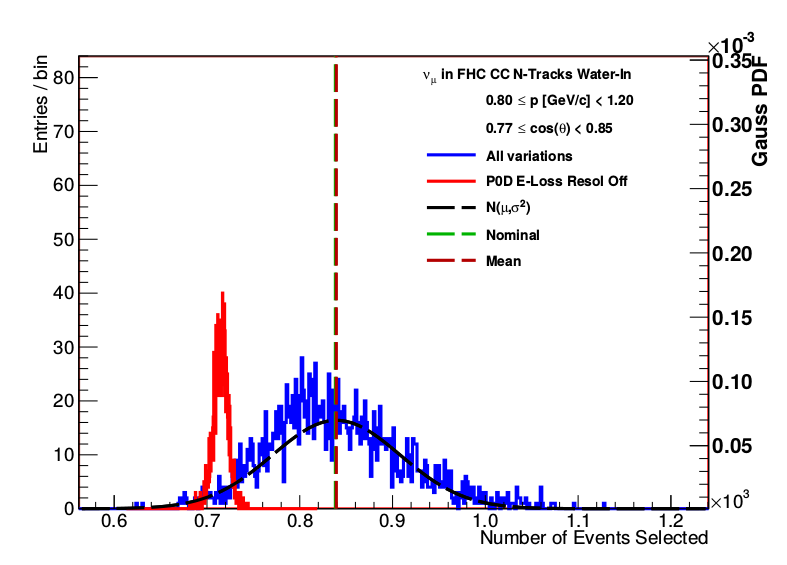
\includegraphics[width=0.445\textwidth]{Chapters/Figures/P0DBANFFParameterization/P0DObsnormSpreadNumuCCNTrks}
\par\end{centering}
}
\par\end{centering}
\begin{centering}
\subfloat[$\protect\numubar$ in RHC CC 1-Track]{\begin{centering}
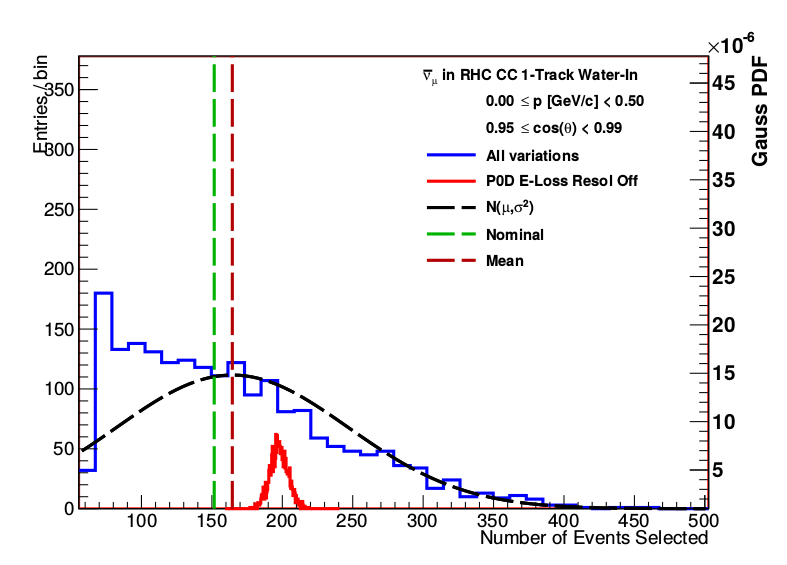
\includegraphics[width=0.445\textwidth]{Chapters/Figures/P0DBANFFParameterization/P0DObsnormSpreadNumubarRHCCC1Trk}
\par\end{centering}
}\subfloat[$\protect\numubar$ in RHC CC N-Tracks]{\begin{centering}
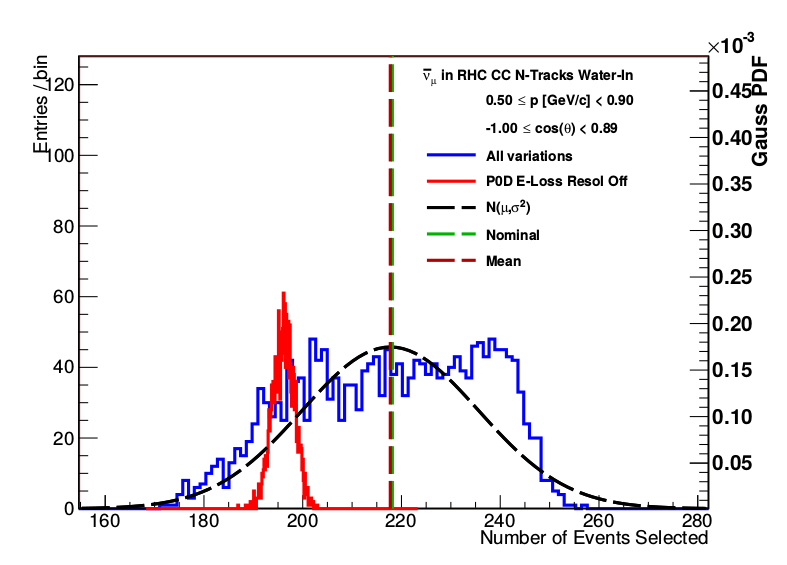
\includegraphics[width=0.445\textwidth]{Chapters/Figures/P0DBANFFParameterization/P0DObsnormSpreadNumubarRHCCCNTrks}
\par\end{centering}
}
\par\end{centering}
\begin{centering}
\subfloat[$\protect\numu$ in RHC CC 1-Track]{\begin{centering}
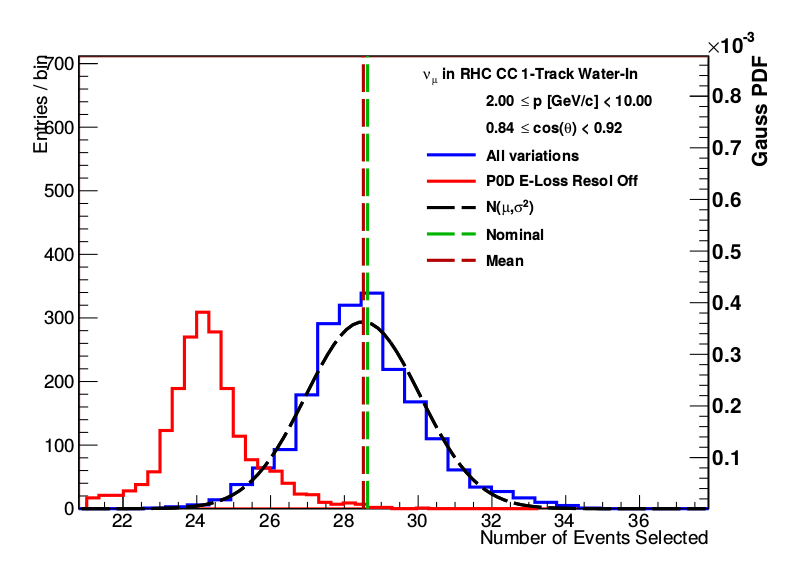
\includegraphics[width=0.445\textwidth]{Chapters/Figures/P0DBANFFParameterization/P0DObsnormSpreadNumuRHCCC1Trk}
\par\end{centering}
}\subfloat[$\protect\numu$ in RHC CC N-Tracks]{\begin{centering}
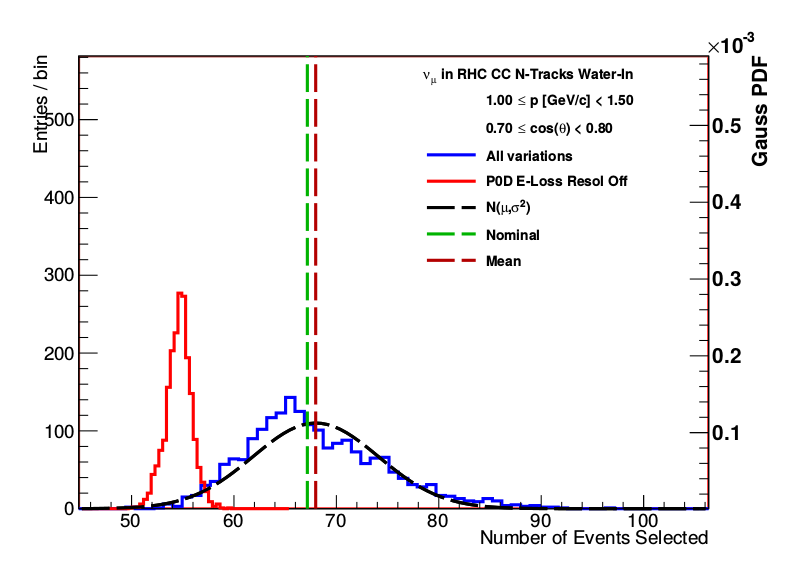
\includegraphics[width=0.445\textwidth]{Chapters/Figures/P0DBANFFParameterization/P0DObsnormSpreadNumuRHCCCNTrks}
\par\end{centering}
}
\par\end{centering}
\caption[Event Variations in Observable Normalization Bins]{Event variations in representative observable normalization bins.
Shown in each sub-figure the varied event rate from all toy experiments
in a particular observable normalization bin. The blue curve has all
the systematics enabled while the red curve has the ELossRes systematic
disabled. Vertical dashed lines show the unvaried, weighted MC prediction
and varied mean of all toy experiments. The ratio of the horizontal
positions of each vertical line is the prefit normalization value
for that bin. A Gaussian with variance extracted from the covariance
matrix is shown to illustrate the bin's estimate on the normalization
uncertainty. \label{fig:Representative-event-variations}}
\end{figure}

The detector systematic that had the largest effect on the observable
normalization prediction was the $\pod$ energy loss resolution (ELossRes)
which alters the amount of particle energy deposited in the $\pod$.
This systematic was developed for the $\numu$ CC-$0\pi$ cross section
analysis, it was identified as the largest detector systematic uncertainty
in the cross section measurement\cite{Yuan2016}. When the deposited
energy in the $\pod$ is varied, it also changes the distance the
truth matched particle travels in the $\pod$. Hence, this systematic
changes the likelihood of a particle being reconstructed as a track.
The observed effect is that for bins with relatively low muon momentum,
the number of predicted events can vary in a non-Gaussian manner as
shown in \prettyref{fig:Representative-event-variations}.

An unexpected phenomenon was observed when comparing the toy experiments
with and without the ELossRes variation applied. With the ELossRes
variation disabled in the toy experiments, a relatively large shift
in the bin prediction was observed compared to the nominal prediction.
This shift was expected, but what was not expected was the direction
of the shift as shown in \prettyref{fig:Representative-event-variations}.
In most cases, the shift is below the nominal MC value. However, in
many of the bins, that the shape location of the prediction is above
the expectation. This behavior was unexpected prior to running the
toy experiment variations.

A relationship between the prediction shape location and selection
purity as a function of $\left(p,\cos\theta\right)$ was discovered.
In high purity $\left(p,\cos\theta\right)$-regions of the 1-Track
samples, the shape location of the prediction in the disabled ELossRes
toy experiments was below the nominal MC prediction. When the 1-Track
sample purity was lower, however, the shape location was above it.
This effect is likely due to events migrating from the 1-Track samples
into the N-Tracks samples due to multiple particles in the event.

The finalized observable normalization bins are listed below. There
are in total $N_{\text{d}}=461$ bin normalization parameters. The
covariance matrix used in the BANFF fit is shown in \prettyref{fig:The-updated-detector-covariance}.
Their respective fit indices, prefit values, and prefit standard deviations
are tabulated in Appendix \prettyref{app:obsnorm}.
\begin{itemize}
\item The $\numu$ in FHC Mode CC 1-Track samples bin normalization edges:
\begin{itemize}
\item $p$ {[}GeV/c{]}: 0, 0.4, 0.6, 0.8, 1.25, 2, 3, 4, 5.5, 30
\item $\cos\theta$: -1, 0.7, 0.8, 0.94, 0.975, 0.99, 1
\end{itemize}
\item The $\numu$ in FHC Mode CC N-Tracks samples bin normalization edges:
\begin{itemize}
\item $p$ {[}GeV/c{]}: 0, 0.4, 0.6, 0.8, 1.2, 2.2, 3.5, 10, 30
\item $\cos\theta$ : -1, 0.77, 0.85, 0.9, 0.97, 1
\end{itemize}
\item The $\numubar$ in RHC Mode CC 1-Track samples bin normalization edges:
\begin{itemize}
\item $p$ {[}GeV/c{]}: 0, 0.5, 0.6, 0.8, 1.25, 2, 3, 30
\item $\cos\theta$ : -1, 0.82, 0.9, 0.95, 0.99, 1
\end{itemize}
\item The $\numubar$ in RHC Mode CC N-Tracks samples bin normalization
edges:
\begin{itemize}
\item $p$ {[}GeV/c{]}: 0, 0.5, 0.9, 1.25, 1.6, 3, 30
\item $\cos\theta$ : -1, 0.89, 0.95, 0.97, 0.99, 1
\end{itemize}
\item The $\numu$ in RHC Mode CC 1-Track samples bin normalization edges:
\begin{itemize}
\item $p$ {[}GeV/c{]}: 0, 0.4, 0.6, 0.8, 1.1, 2, 10
\item $\cos\theta$ : -1, 0.78, 0.84, 0.92, 0.95, 0.98, 0.99, 1
\end{itemize}
\item The $\numu$ in RHC Mode CC N-Tracks samples bin normalization edges:
\begin{itemize}
\item $p$ {[}GeV/c{]}: 0, 0.6, 1, 1.5, 2, 10
\item $\cos\theta$ : -1, 0.7, 0.8, 0.85, 0.98, 0.99, 1
\end{itemize}
\end{itemize}
\begin{figure}
\begin{centering}
\subfloat[Covariance matrix]{\begin{centering}
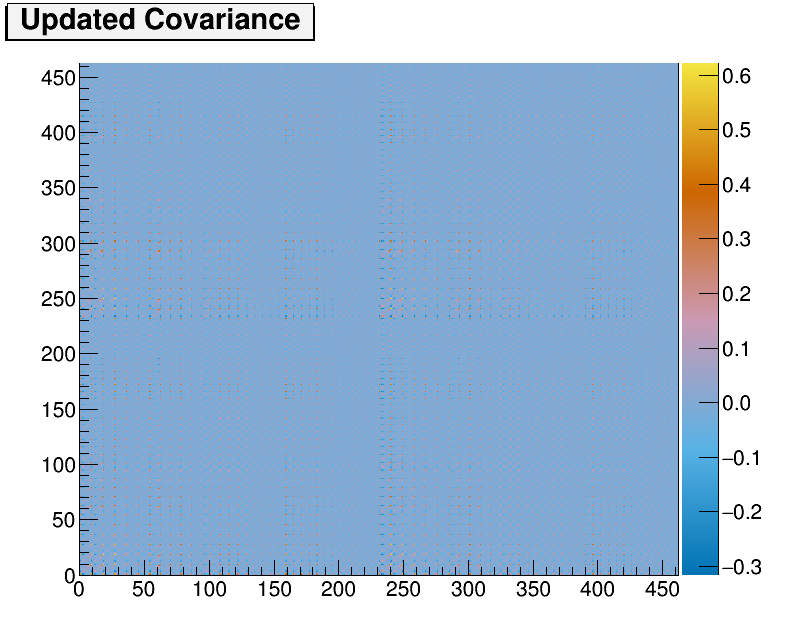
\includegraphics[height=0.4\textheight]{Chapters/Figures/P0DBANFFParameterization/P0DMass_TPCMatch_study/obsNorm_cov_updated}
\par\end{centering}
}
\par\end{centering}
\begin{centering}
\subfloat[Correlation matrix]{\begin{centering}
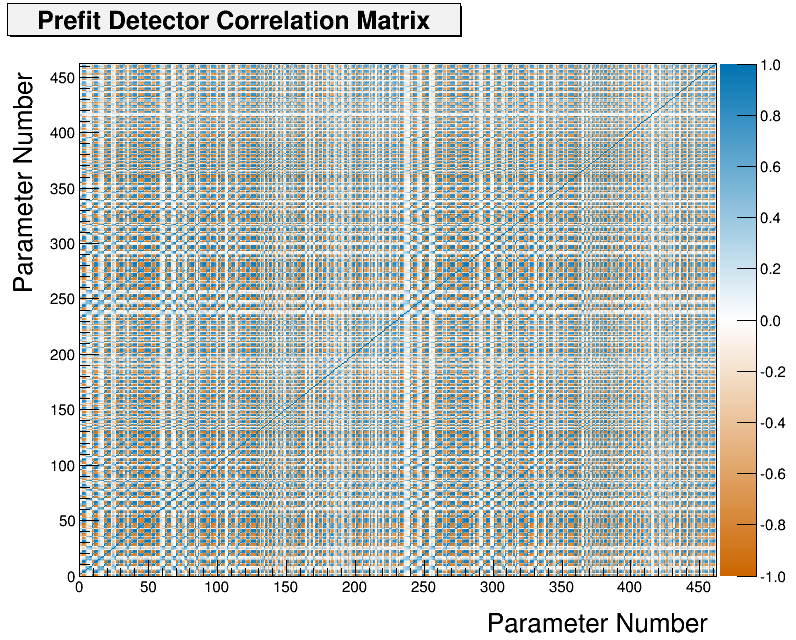
\includegraphics[height=0.4\textheight]{Chapters/Figures/P0DBANFFParameterization/corr_dete_pref}
\par\end{centering}
}
\par\end{centering}
\caption[Detector Penalty Covariance Matrix]{Detector penalty covariance matrix. Shown in figure (a) is covariance
matrix and (b) is the correlation matrix. Note that the parameter
indices, which represent the bin normalization indices, are offset
from their fit indices value by 99. \label{fig:The-updated-detector-covariance}}
\end{figure}

To better understand how effective the choice of bin normalizations
parameters are at characterizing the data variance, principal component
analysis was performed using all the available toy experiments. Principal
component analysis is the process of a eigenvalue decomposition of
a square matrix, $M$. The principal components of $M$, which describe
the data variance, are the eigenvectors. The relative importance of
each eigenvector is set by the magnitude of the associated eigenvalue.

Using this prescription, we define the sample variance, $S$, as
\[
S=\frac{1}{N_{\text{toys}}}X^{T}X,
\]
where $X$ is a $N_{\text{toys}}\times N_{\text{d}}$ matrix of the
predicted number of events (not the normalization!) in each normalization
bin. The eigenvalue decomposition of $S$ is given by
\[
S=U^{T}\Lambda U,
\]
where $U$ is the eigenvector matrix of $S$ and $\Lambda$ is a diagonal
matrix of the $S$ matrix eigenvalues. What is useful using principal
component analysis is that the eigenvalues and eigenvectors are sorted
from largest to smallest magnitude. The sample variance eigenvalues
are shown in \prettyref{tab:Eigenvalues-sample-covariance}. The first,
and hence largest, eigenvalue is two orders of magnitude larger than
the next largest eigenvalue, which means that the majority of the
bin-to-bin variance can be explained by the first eigenvector. The
first eigenvector's coefficients are shown in \prettyref{fig:Principal-components}.
We see that all the components are negative and clustered. This result
is interpreted to mean we can expect the bins normalizations postfit
values to shift all together uniformly.

\begin{table}
\caption[Eigenvalues of the Sample Covariance]{Eigenvalues of the sample covariance. The values are sorted from largest
to smallest in magnitude. Note that the parameter indices, which represent
the bin normalization indices, are offset from their fit indices value
by 99.\label{tab:Eigenvalues-sample-covariance}}

\begin{centering}
\begin{tabular}{|c||c|c|c|c|c|c|c|c|c|}
\hline 
Index & 0 & 1 & 2 & 3 & \ldots{} & 458 & 459 & 460 & 461\tabularnewline
Eigenvalue & 2029 & 16.45 & 12.87 & 11.10 & \ldots{} & 0.05325 & 0.05129 & 0.04955 & 0.03992\tabularnewline
\hline 
\end{tabular}
\par\end{centering}
\end{table}

\begin{figure}
\begin{centering}
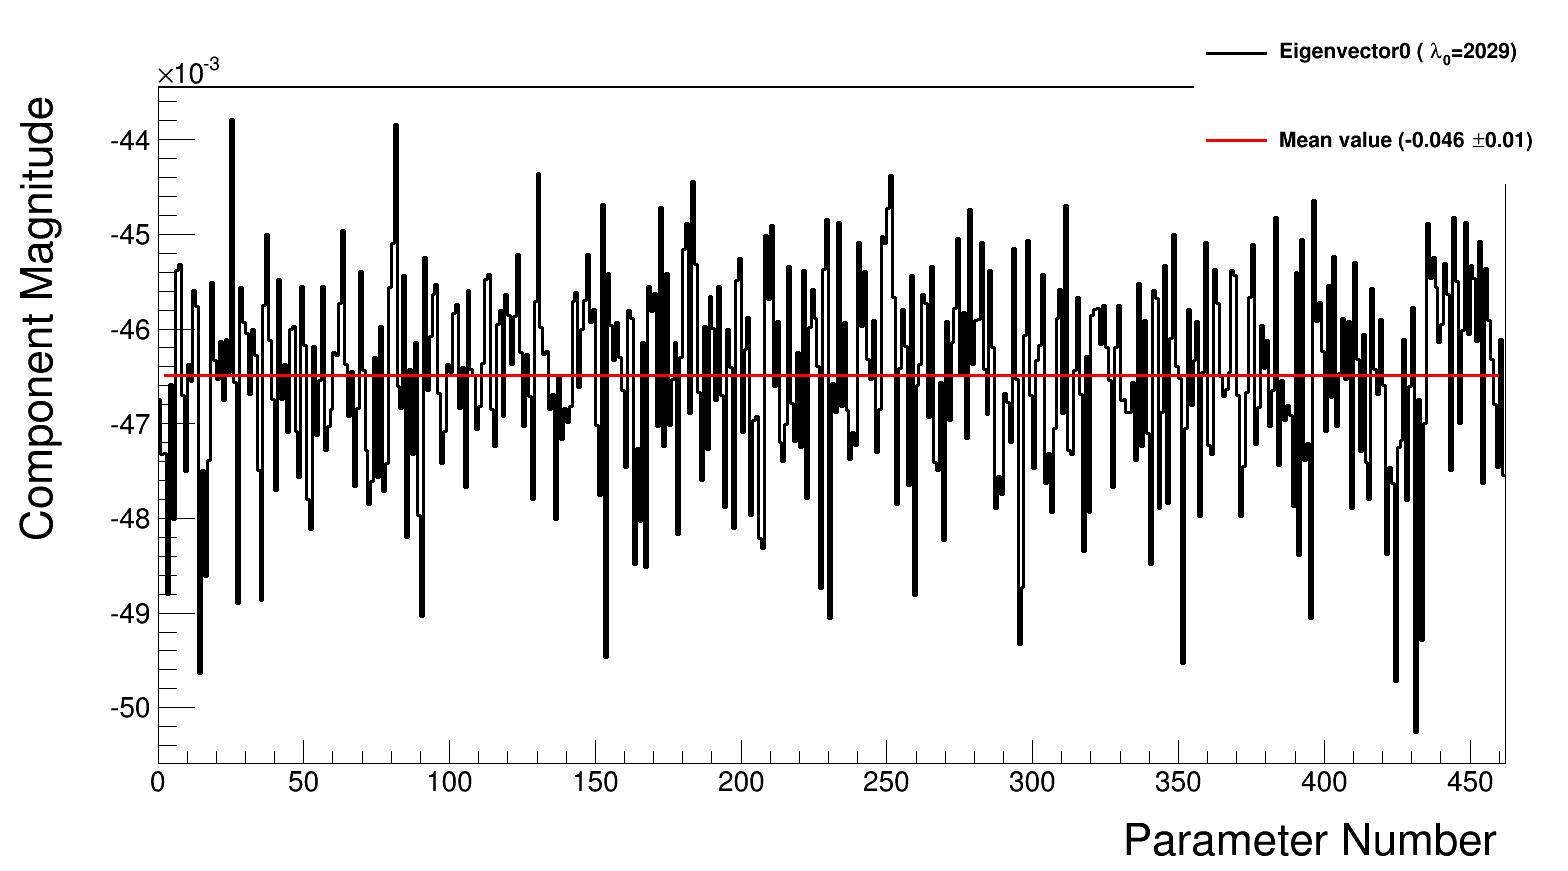
\includegraphics[width=0.98\textwidth]{Chapters/Figures/P0DBANFFParameterization/EigenVector0}
\par\end{centering}
\caption[Principal Component for the Sample Variance]{Principal component for the sample variance. This is the eigenvector
associated with the largest eigenvalue of magnitude. Each parameter
coefficient refers to the slope of the axis that describes most of
the variance in the sample. The coefficients are all negative and
are of similar magnitude. Together, they suggest all the normalization
parameters respond linearly and uniformly. Note that the parameter
indices, which represent the bin normalization indices, are offset
from their fit indices value by 99.\label{fig:Principal-components}}

\end{figure}

Additionally, we can estimate the effective degrees of freedom for
the bin normalization parameters. The effective degrees of freedom
is given by
\begin{equation}
\text{df}(r)=\sum_{i=0}^{N_{\text{d}}}\frac{\lambda_{i}}{\lambda_{i}+r},\label{eq:effective-degrees-of-freedom}
\end{equation}
where $\lambda_{i}$ are the eigenvalues of $\Lambda$ and $r$ is
a tunable parameter\cite{springer_series978-0-387-84858-7}. The idea
behind \eqref{eq:effective-degrees-of-freedom} is that although all
$N_{\text{d}}$ coefficients will be non-zero, they are restricted
to vary by the magnitude of $r$. In particular, $r$ represents the
regularization strength for the detector systematics penalty, which
is set to one ($r=1$) in the BANFF fit. If there was no (regularization)
penalty, or $r=0$, then the number of degrees of freedom is df(0)=$N_{d}$.
It is found that there are about 137 effective degrees of freedom
for the bin normalization parameters, or 29\% of $N_{\text{d}}$.
This suggests that a much smaller number bin normalization parameters
can effectively describe the sample variance. This is particularly
important to consider for a future BANFF fit analysis since this can
provide a computational performance while maintaining predictability
power in the ND constraint measurement. No further reduction in the
number of bin normalization parameters were pursued due to time constraints.


\subsection{Cross Section Model}

There are a number of neutrino-nucleus interaction model parameters
implemented in the BANFF fit to account for the uncertainties in cross
section measurements. They are frequently updated to account for new
models and constraints from external data. The cross section models
used in this analysis use the T2K 2017 parameterization, which is
a canonical set of parameters shared among all analyses in T2K. A
gross description of the cross section model is provided here with
a full description in the following reference\cite{PhysRevLett.121.171802}.

There are three types of cross section parameters: shape, normalization,
and functional. A cross section shape parameter, $x^{\text{Shape}}$,
is defined as a shift in the location of a certain feature in the
cross section. The shape parameters are stored in one dimensional
splines 
\[
w\left(x^{\text{Shape}}\right)=\frac{d^{n}\sigma\left(x^{\text{Shape}}\right)}{dz^{n}}/\frac{d^{n}\sigma\left(x_{0}^{\text{Shape}}\right)}{dz^{n}},
\]
where $d^{n}\sigma/dz^{n}$ is a $n$ dimensional cross section of
$z$ dependent parameters, and $x_{0}^{\text{Shape}}$ is the nominal
value of the shape parameter. As a design choice, the shape location
parameters all start with a prefit value of zero (0). A cross section
normalization parameter, $x_{i}^{\text{Norm}}$, is defined as
\begin{equation}
x^{\text{Norm}}=\frac{p^{\prime}}{p},\label{eq:xsecnormdef}
\end{equation}
where $p$ and $p^{\prime}$ are NEUT nominal and ND constrained parameters,
respectively. And finally functional parameters are scalars to model
a cross section function of a true kinematic. For example, if a cross
section is given by $\sigma(x)=mx+b$, $m$ and $b$ are the functional
parameters in the model. Combining these parameters into a single
vector $\vec{x}$, the cross section penalty term, $\chi_{\text{Det}}^{2}$,
is given by
\[
\chi_{\text{Det}}^{2}=\left(\vec{x}-\vec{x}_{0}\right)^{T}\left(V^{\text{xsec}}\right)^{-1}\left(\vec{x}-\vec{x}_{0}\right),
\]
where $\vec{x}_{0}$ is the initial values of the cross section parameters,
and $V^{\text{xsec}}$ is the cross section model covariance matrix.

The next sections deal with the model parameterizations and systematic
uncertainties in the NEUT version 5.3.3\cite{Wret2019} interaction
library which is used in T2K MC and oscillation analysis.

\subsubsection{The CC-0\pititle{} Model}

The cross section models with the largest impact on T2K's oscillation
sensitivity are CCQE and CCQE-like interactions, collectively called
CC-0$\pion$. At energies near the $\nue$ appearance maximum, $E_{\nu}=0.6$
GeV, the CCQE interaction is the largest contributor to the neutrino
cross section as shown in \prettyref{fig:PredictedCCincxsec}. The
nominal CCQE model in NEUT is a Spectral Function (SF) from Benhar
\textit{et al}\cite{Benhar:1995}. \textcolor{black}{An alternative
CCQE model incorporates the Llewellyn-Smith dipole axial form factor}\footnote{A form factor is a measure of scattering amplitude in the form of
the Fourier transform of some charge distribution.}\cite{PhysRev.141.1298,LlewellynSmith:1971uhs} and BBBA05 vector
form factors coupled to a Smith-Moniz Relativistic Fermi Gas\cite{SMITH1972605,Niewczas:2015iea,Bradford2006}
(RFG). A CCQE-like excitation mode involves correlated nucleon pair
scattering called ``2 particle, 2 hole''\cite{Martini:2009uj} (2p2h).
An additional nuclear model called the ``Random Phase Approximation''
(RPA)\cite{Co:2006wnm,Nieves:2011pp} is used to to modify single
nucleon scattering by accounting for nucleon correlations inside the
nucleus. The default CC-$0\pi$ model for T2K analyses is the combination
of the \textcolor{black}{Llewellyn-Smit}h+RFG model, 2p2h excitation,
and RPA nuclear model. This combination was selected due to poor data
matching with the SF model\cite{Wret2019}.

The CC-$0\pi$ model has three CCQE parameters: the dipole axial form
factor mass $M_{A}^{\text{QE}}$ from the \textcolor{black}{Llewellyn-Smith}
model, and two Fermi momentum parameters $p_{F}$, one for \ce{^{12}C}
and one for \ce{^{16}O} that describe the momentum of nucleons on
the surface of a RFG. In the past, using these parameters has been
shown to work as effective parameters in T2K when unconstrained. In
this analysis, these three parameter are unconstrained. In other words,
a flat prior is used for $M_{A}^{\text{QE}}$, $p_{F}^{C}$, and $p_{F}^{O}$.

For the 2p2h excitation, there are a total of five parameters to describe
the model. Three are normalization terms: the $\nu$ interaction on
\ce{^{12}C}, the $\antinu$ interaction on \ce{^{12}C}, and the
scaling for \ce{^{12}C}$\rightarrow$\ce{^{16}O}. The remaining
two systematic parameters in the 2p2h excitation are shape parameters,
one for \ce{^{12}C} and one for \ce{^{16}O}. They are used constrain
the interplay of the contributing modes in 2p2h. One contributing
mode is the Meson Exchange Current (MEC) which involves a virtual
meson exchange between the nucleons. The other mode is nucleon-nucleon
(NN) correlations which involves virtual particle exchange. A shape
value of -1 determines 2p2h is completely due to MEC, 0 is the nominal
MC 2p2h model, and +1 determines 2p2h is completely due to NN. Any
differences in the event rate in the region between $\pm1$ is absorbed
by a interference term. However, since no existing T2K nor external
neutrino data can constrain the neutrino-induced 2p2h interaction,
a flat prior is set for all 2p2h parameters.

The other nuclear interaction in the CC-$0\pi$ model uses the Nieves
RPA model\cite{Nieves:2011pp} to describe nucleon correlations. The
RPA model primarily alters the single nucleon cross section and has
dependence on both $E_{\nu}$ and $Q^{2}$. A functional weighting
scheme called ``BeRPA'' having only $Q^{2}$ dependence was found
to work well to mimic the inherent uncertainties in the Nieves RPA
model. The BeRPA functional is given by
\begin{equation}
w\left(Q^{2}\right)=\begin{cases}
A\beta_{0}^{3}\left(x\right)+B\beta_{1}^{3}\left(x\right)+p_{1}\beta_{2}^{3}\left(x\right)+D\beta_{3}^{3}\left(x\right) & Q^{2}\leq U\\
1+p_{2}\exp\left(-E\left[Q^{2}-U\right]\right), & Q^{2}>U
\end{cases}\label{eq:BeRPA}
\end{equation}
where $x=Q^{2}/U$, $\beta_{i}^{n}\left(x\right)$ are the Bernstein
polynomials\cite{FAROUKI2012379} 
\begin{equation}
\beta_{i}^{n}\left(x\right)=\binom{n}{i}x^{i}\left(1-x\right)^{n-i}\quad x\in[0,1],\label{eq:BernsteinBasis}
\end{equation}
$p_{1}$ and $p_{2}$ absorb the continuity conditions, 
\begin{equation}
p_{1}=D+\frac{UE\left(D-1\right)}{3},\quad p_{2}=D-1,\label{eq:BeRPAContinuity}
\end{equation}
and $A$, $B$, $D$, $E$, and $U$ are the functional parameters.
The parameter $U$ is fixed to prevent unwieldy correlations from
appearing.

\subsubsection{The CC-$1$\pititle{} Model}

Another important exclusive channel in NEUT is resonance states that
produce a single pion or CC-$1\pi$. The CC-$1\pi$ model incorporates
the Rein-Seghal model of neutrino-induced $\Delta$ resonance decay\cite{PhysRevD.90.093001,Graczyk:2009qm,PhysRevD.77.053001,rein-sehgal}
with lepton mass corrections\cite{PhysRevD.77.053003,PhysRevD.76.113004}.
There are just three tunable parameters in the model. They are resonant
axial mass $M_{A}^{\text{Res}}$, the axial form factor normalization
$C_{A}^{5}$, and the isospin=$\nicefrac{1}{2}$ $\left(I_{1/2}\right)$
background normalization. These three parameters are known to effectively
describe neutrino-induced single pion production data from Brookhaven
National Laboratory\cite{PhysRevD.34.2554} and Argonne National Laboratory\cite{PhysRevD.25.1161}.
It is important to know that $M_{A}^{\text{Res}}$ and $C_{A}^{5}$
are strongly anticorrelated due to the parameterization of the form
factor
\begin{equation}
f\left(Q^{2}\right)=C_{A}^{5}\left(1+\frac{Q^{2}}{\left(M_{A}^{\text{Res}}c^{2}\right)^{2}}\right)^{-2}.\label{eq:CC1piaxialformfactor}
\end{equation}


\subsubsection{Coherent Pion Production}

Coherent scattering refers to scattering where the wavelength of the
incoming particle is larger than the target. In the case of coherent
neutrino-nucleus scattering, the neutrino's de Broglie wavelength
is larger than the size of the nucleus. In the scattering, no quantum
numbers are exchanged, but the nucleus experiences a momentum boost.
In coherent pion production, the in-flight virtual boson is converted
into a pion with that pion exchanging a Pomeron\cite{Abe2016} with
the nucleus. The coherent scattering model is described by Rein-Sehgal
\cite{REIN198329}. Lookup tables are used to scale the cross section
to external data\cite{Wret2019} and the Berger-Sehgal model \cite{PhysRevD.76.113004}.
Three tunable normalization parameters are used describe the coherent
production model: CC on \ce{^{12}C}, CC on \ce{^{16}O}, and NC on
all nuclei. As a design choice, both CC parameters are 100\% correlated
with one another, meaning that any change in one parameter changes
the other identically.

\subsubsection{High Energy Scattering Model}

There are two parameters that describe high energy neutrino scattering.
One is a CC deep inelastic scattering (DIS) interaction shape parameter
called ``CC DIS''. The other is a normalization for NC interactions
called ``NC Other''. The CC DIS parameter, which also includes multiple
pion production, is modeled as a function of $E_{\nu}$ with a simple
uncertainty relation of 
\[
\frac{0.4}{\Enu\text{ [GeV]}}(\%),
\]
where the uncertainty at 4.0 GeV is 10\%. The NC Other parameter is
a normalization on NC DIS, single kaon production, single $\eta$-meson
production, and NC elastic processes with a flat 30\% fractional uncertainty\cite{Wret2019}.

\subsubsection{Final State Interactions}

Final state interactions\cite{Golan:2012wx} (FSI) are effects that
alter final state pions from neutrino-nucleus events before the pion
exits the nucleus. The microscopic model in NEUT is a cascade implementation
of the Salcedo-Oset model\cite{SALCEDO1988557} which describes interactions
in the nucleus as probabilities of position and momentum tuned to
the world data\cite{PhysRevC.18.584}. These processes are divided
into six classes with one parameter for each. These classes are the
low energy inelastic scattering (INEL), high energy INEL, pion absorption
(ABS), pion production (PROD), low energy charge exchange (CEX), and
high energy CEX. The low and high energy transition for both the inelastic
scattering and charge exchange processes occurs at $p_{\pi}=500$
MeV/c.

\subsubsection{Fixed Parameters}

As mentioned in the CC-$0\pi$ model, the BeRPA $U$ parameter is
fixed to minimize correlations with the other BeRPA scale parameters.
However, there are four other fixed normalization parameters in the
BANFF fit since they correspond to SK only parameters. They are included
in the fit in order to maintain consistency between the ND280 constraint
and oscillation analysis parameterizations. In other words, they are
spectators in the BANFF fit. These parameters are the CC $\nue$/$\numu$
event rate ratio, CC $\nuebar$/$\numubar$ event rate ratio, NC-$1\gamma$
event rate, and NC other far detector event rate.

\subsubsection{Prefit Values and Covariance Matrix}

There are a total of 31 cross section parameters in the BANFF fit,
five of which are fixed. The fit parameters are listed in \prettyref{tab:Cross-Section-Model}
with the associated covariance matrix shown in \prettyref{fig:Cross-section-correlations-prefit}.
Following the definition of the flux and bin normalization parameters,
cross section parameters are defined as fractional differences either
in shape, scale, or normalization. If no prefit uncertainty is shown
in \prettyref{tab:Cross-Section-Model}, and emphasized using \textcolor{red}{red
font}, then the parameter had a flat prior assigned. A model parameter
with an asterisk $\left(^{*}\right)$ next to it is fixed in the fit.
Abbreviations used in this table are ``dim.-less'' for dimensionless,
``norm.'' for normalization, ``Near'' for ND280, ``Far'' for
Super-Kamiokande, and ``bkg'' for background. Parameters with physical
units are shown in both dimensionless and dimensional values for comparison.
Prefit values are relative to the NEUT nominal value.

\begin{figure}
\begin{centering}
\subfloat[Covariance matrix]{\begin{centering}
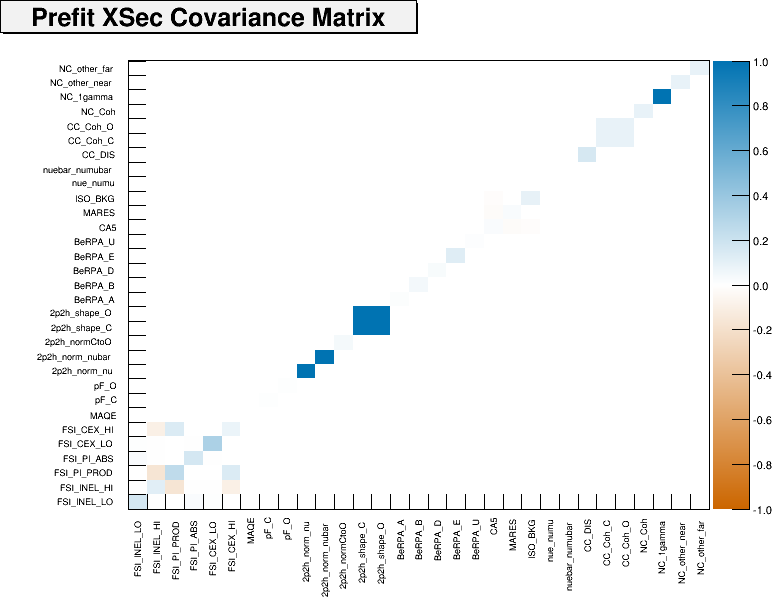
\includegraphics[height=0.4\textheight]{Chapters/Figures/P0DBANFFParameterization/cov_xsec_pref}
\par\end{centering}

}
\par\end{centering}
\begin{centering}
\subfloat[Correlation correlation]{\begin{centering}
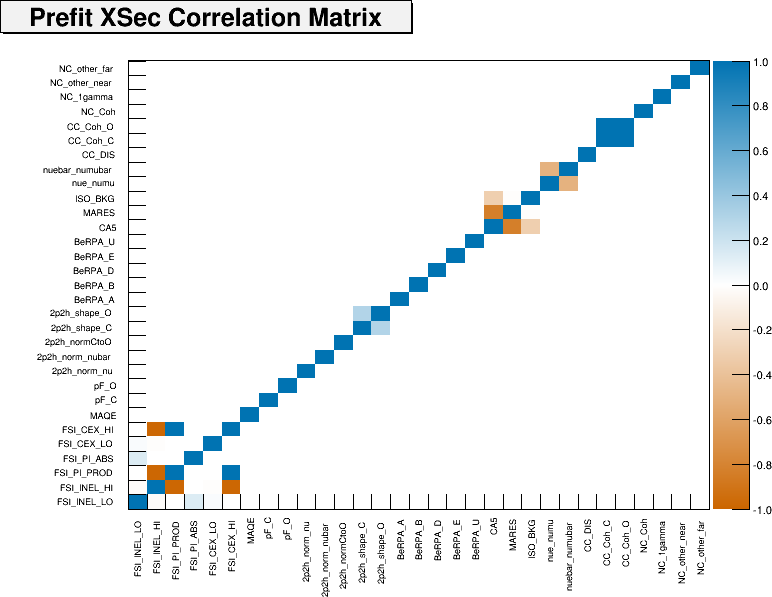
\includegraphics[height=0.4\textheight]{Chapters/Figures/P0DBANFFParameterization/corr_xsec_pref}
\par\end{centering}
}
\par\end{centering}
\caption[Cross Section Parameters Prefit Covariance and Correlation Matrices]{Cross section parameters prefit covariance and correlation matrices.
\label{fig:Cross-section-correlations-prefit}}
\end{figure}

\begin{center}
\begin{longtable}[c]{|c|c|c|c|c|}
\hline
\caption[Cross Section Model Fit Parameters in the BANFF Fit]{Cross section model parameters in the fit. See the text for a full
description. \label{tab:Cross-Section-Model}}
\tabularnewline
\hline 
\textbf{Fit index} & \textbf{Topology} & \textbf{Model} & \textbf{Parameter} & \textbf{Prefit}\tabularnewline
\hline
\endfirsthead
\hline
\hline 
\textbf{Fit index} & \textbf{Topology} & \textbf{Model} & \textbf{Parameter} & \textbf{Prefit}\tabularnewline
\hline
\endhead
562 & All & FSI & Low energy INEL & $0\pm0.41$\tabularnewline
\cline{1-1} \cline{4-5} \cline{5-5} 
563 &  &  & High energy INEL & $0\pm0.34$\tabularnewline
\cline{1-1} \cline{4-5} \cline{5-5} 
564 & \multirow{2}{*}{} &  & PROD & $0\pm0.41$\tabularnewline
\cline{1-1} \cline{4-5} \cline{5-5} 
565 &  &  & ABS & $0\pm0.5$\tabularnewline
\cline{1-1} \cline{4-5} \cline{5-5} 
566 &  &  & Low energy CEX & $0\pm0.57$\tabularnewline
\cline{1-1} \cline{4-5} \cline{5-5} 
567 &  &  & High energy CEX & $0\pm0.28$\tabularnewline
\hline 
\multirow{2}{*}{\textcolor{red}{568}} & \textcolor{black}{CC-$0\pi$} & \textcolor{red}{Llewellyn-} & \textcolor{red}{$M_{A}^{\text{QE}}$ (dim.-less)} & \textcolor{red}{$1$}\tabularnewline
 &  & \textcolor{red}{Smith} & \textcolor{red}{$M_{A}^{\text{QE}}$ $\left(\text{GeV/}\csq\right)$} & \textcolor{red}{$1.20$}\tabularnewline
\cline{1-1} \cline{3-5} \cline{4-5} \cline{5-5} 
\multirow{2}{*}{\textcolor{red}{569}} &  & \textcolor{red}{RFG} & \textcolor{red}{$p_{F}^{C}$ (dim.-less)} & \textcolor{red}{$1$}\tabularnewline
 &  & \multirow{2}{*}{} & \textcolor{red}{$p_{F}^{C}$ $\left(\text{MeV/c}\right)$} & \textcolor{red}{$217$}\tabularnewline
\cline{1-1} \cline{4-5} \cline{5-5} 
\multirow{2}{*}{\textcolor{red}{570}} &  &  & \textcolor{red}{$p_{F}^{O}$ (dim.-less)} & \textcolor{red}{$1$}\tabularnewline
 &  &  & \textcolor{red}{$p_{F}^{O}$ $\left(\text{MeV/c}\right)$} & \textcolor{red}{$225$}\tabularnewline
\cline{1-1} \cline{3-5} \cline{4-5} \cline{5-5} 
\textcolor{red}{571} &  & \textcolor{red}{Nieves 2p2h} & \textcolor{red}{$\nu$ norm. on \ce{^{12}C}} & \textcolor{red}{$1$}\tabularnewline
\cline{1-1} \cline{4-5} \cline{5-5} 
\textcolor{red}{572} &  &  & \textcolor{red}{$\antinu$ norm. on \ce{^{12}C}} & \textcolor{red}{$1$}\tabularnewline
\cline{1-1} \cline{4-5} \cline{5-5} 
\textcolor{red}{573} &  &  & \textcolor{red}{\ce{^{12}C}$\rightarrow$\ce{^{16}O} norm.} & \textcolor{red}{$1$}\tabularnewline
\cline{1-1} \cline{4-5} \cline{5-5} 
\textcolor{red}{574} &  &  & \textcolor{red}{\ce{^{16}C} shape location} & \textcolor{red}{$0$}\tabularnewline
\cline{1-1} \cline{4-5} \cline{5-5} 
\textcolor{red}{575} &  &  & \textcolor{red}{\ce{^{12}O} shape location} & \textcolor{red}{$0$}\tabularnewline
\cline{1-1} \cline{3-5} \cline{4-5} \cline{5-5} 
576 &  & BeRPA & $A$ & $0.59\pm0.118$\tabularnewline
\cline{1-1} \cline{4-5} \cline{5-5} 
577 &  &  & $B$ & $1.05\pm0.21$\tabularnewline
\cline{1-1} \cline{4-5} \cline{5-5} 
578 &  &  & $D$ & $1.13\pm0.1695$\tabularnewline
\cline{1-1} \cline{4-5} \cline{5-5} 
579 &  &  & $E$ & $0.88\pm0.352$\tabularnewline
\cline{1-1} \cline{4-5} \cline{5-5} 
580 &  &  & $U$$^{*}$ & $1.2\pm0.1$\tabularnewline
\hline 
581 & CC-$1\pi$ & Rein-Seghal & $C_{A}^{5}$ & $0.96\pm0.148$\tabularnewline
\cline{1-1} \cline{4-5} \cline{5-5} 
\multirow{2}{*}{582} &  & resonant $1\pi$ & $M_{A}^{\text{Res}}$ (dim.-less) & $1.1263\pm0.157$\tabularnewline
 &  & prodction & $M_{A}^{\text{Res}}$ $\left(\text{GeV/}\csq\right)$ & $1.07\pm0.15$\tabularnewline
\cline{1-1} \cline{4-5} \cline{5-5} 
583 &  &  & $I_{1/2}$ bkg. norm. & $0.74\pm0.307$\tabularnewline
\hline 
584 & Other & Event rate & CC-$\nicefrac{\nue}{\numu}$$^{*}$ & $1\pm0.0282$\tabularnewline
\cline{1-1} \cline{4-5} \cline{5-5} 
585 &  & at SK & CC-$\nicefrac{\antinue}{\antinumu}$$^{*}$ & $1\pm0.0282$\tabularnewline
\cline{1-1} \cline{3-5} \cline{4-5} \cline{5-5} 
586 &  &  & CC DIS shape location & $0\pm0.4$\tabularnewline
\cline{1-1} \cline{3-5} \cline{4-5} \cline{5-5} 
587 &  & Coherent & CC norm. on \ce{^{12}C} & $1\pm0.3$\tabularnewline
\cline{1-1} \cline{4-5} \cline{5-5} 
588 &  & pion & CC norm. on \ce{^{16}O} & $1\pm0.3$\tabularnewline
\cline{1-1} \cline{4-5} \cline{5-5} 
589 &  & production & NC norm. & $1\pm0.3$\tabularnewline
\cline{1-1} \cline{3-5} \cline{4-5} \cline{5-5} 
590 &  & Event rate & NC-1$\gamma$$^{*}$ & $1\pm1$\tabularnewline
\cline{1-1} \cline{4-5} \cline{5-5} 
591 &  &  & NC Other Near & $1\pm0.3$\tabularnewline
\cline{1-1} \cline{4-5} \cline{5-5} 
592 &  &  & NC Other Far$^{*}$ & $1\pm0.3$\tabularnewline
\hline 
\end{longtable}
\par\end{center}


\section{Summary\label{sec:ParameterizationSummary}}

This chapter has described all the fit bins and parameters that go
into the BANFF fit. For the fit bins, they are used in the LLR term
to model the best possible fit between data and MC without any constraints.
However, since there are known systematic uncertainties in the flux,
detector inefficiencies, and cross sections, we have described their
parameterizations to force the fit work within those constraints.
The flux model is constrained by T2K primary and secondary beamline
data while the cross sections are constrained by external data. Finally,
the detector systematics are determined via an ensemble of toy experiments
based on well established control samples in the ND280 detector.

The next chapter describe the set of validation studies used to examine
how the BANFF fit performs.
